%%%%%%%%%%%%%%%%%%%%%%%%%%%%%%%%%%%
% CHAPTER 5: Results + Discussion %
%%%%%%%%%%%%%%%%%%%%%%%%%%%%%%%%%%%
%................................
% Notes about things to add/edit 
%................................
% >> Add plots of gas data stochiometric stuff+
% >> Evaluate comparison of HF and Velocity data and decide if it should be included
% >> Average velocity along entire door?{}
% >> Flame height via video footage?
% >> Linear plots of parameters vs. each other
%%%%%%%%%%%%%%%%%%%%%%%%%%%%%%%%%%%%%%%%%%%%%%%%%%%%%%%%%%%%%%%%%%%%%
\renewcommand{\thechapter}{5}

\chapter{Results and Discussion}
\label{chap:results_disc}
Three different types of figures are presented in this chapter to assist with the discussion of the results. One type is presented with the discussion of the mesh sensitivity study results that were used to select an appropriate grid cell size for the simulations. The other two types are presented throughout the comparison of the predicted data output by the FDS simulations to the corresponding experimental data. 

\section{Mesh Sensitivity Studies}
\label{sec:mesh_studies}
Figures~\ref{fig:east_O2_sensitivity}--\ref{fig:west_cjet_sensitivity} show the oxygen volume fractions and ceiling jet temperatures output by FDS simulations of Test~4 and Test~25 using the coarse, medium, and fine grid sizes across the computational domain.
\begin{figure}[!h]
	\centering
	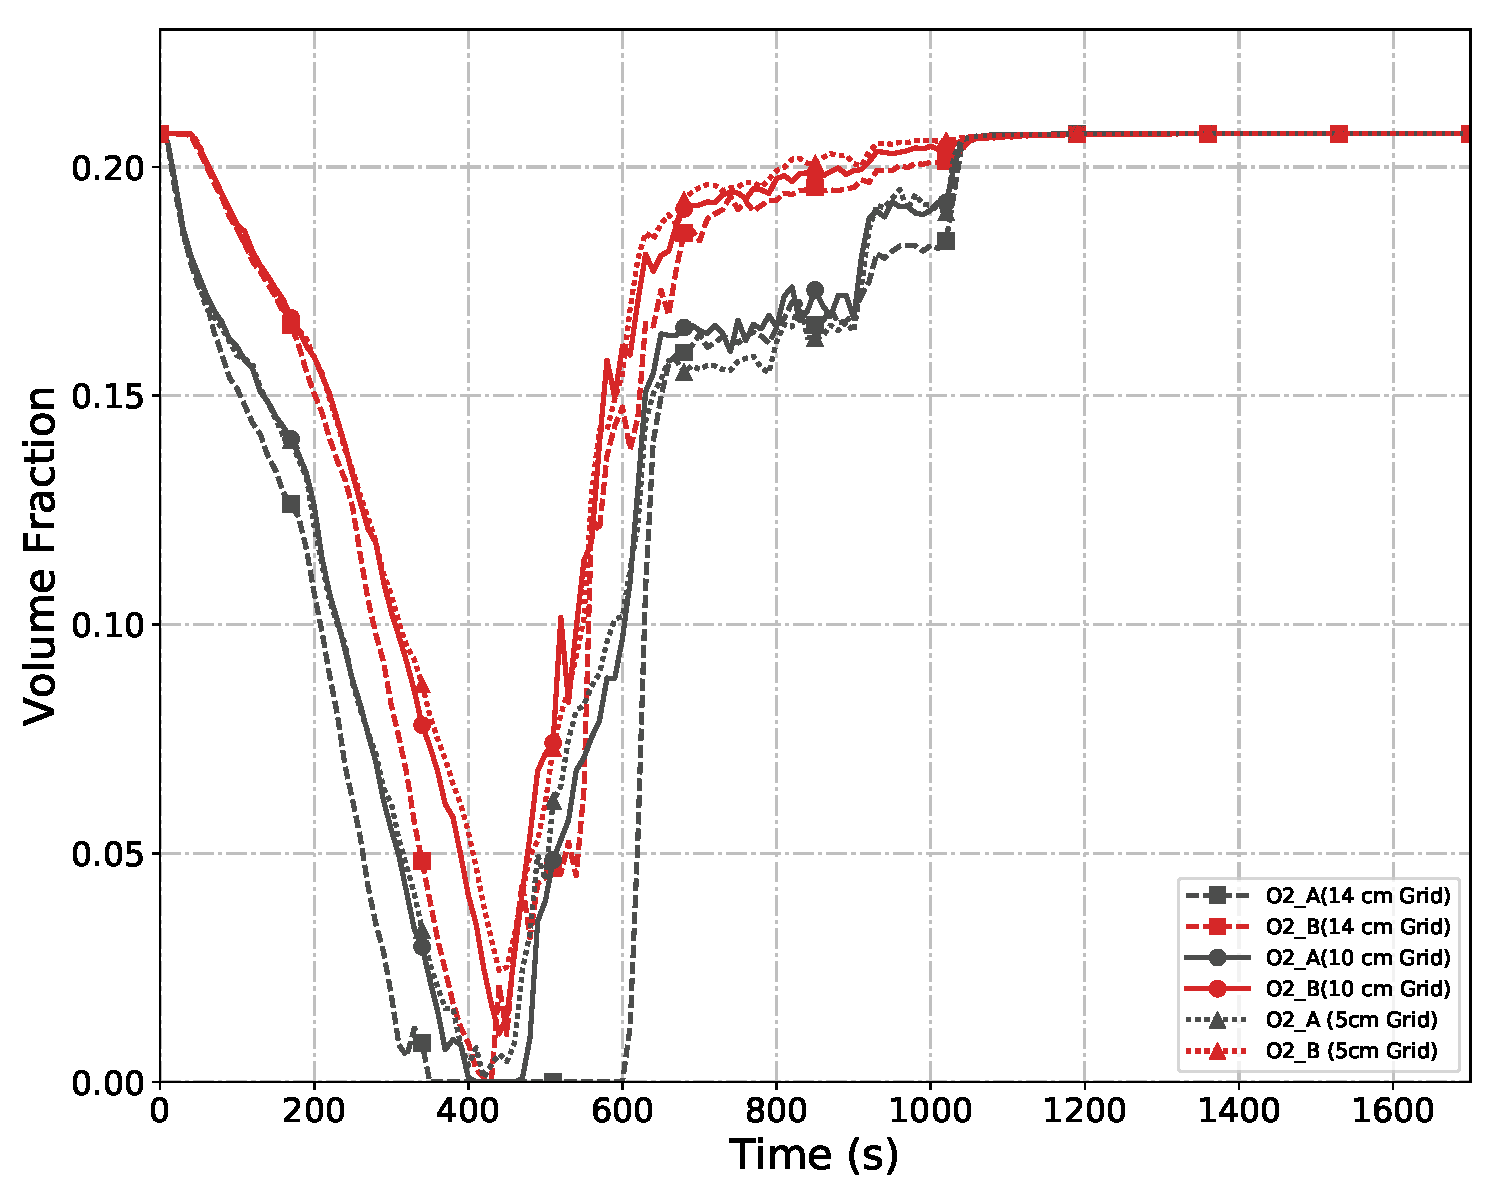
\includegraphics[width=\columnwidth]{Figures/Plots/Grid_Sensitivity/Gas_Concentration/Test_04_O2}
	\caption[$O_2$ concentrations for East Structure simulation with different grid cell sizes.]{$O_2$ concentrations output by the FDS simulation of Test~4 in the East Structure using three different grid cell sizes.}
	\label{fig:east_O2_sensitivity}
\end{figure}

\begin{figure}[!h]
	\centering
	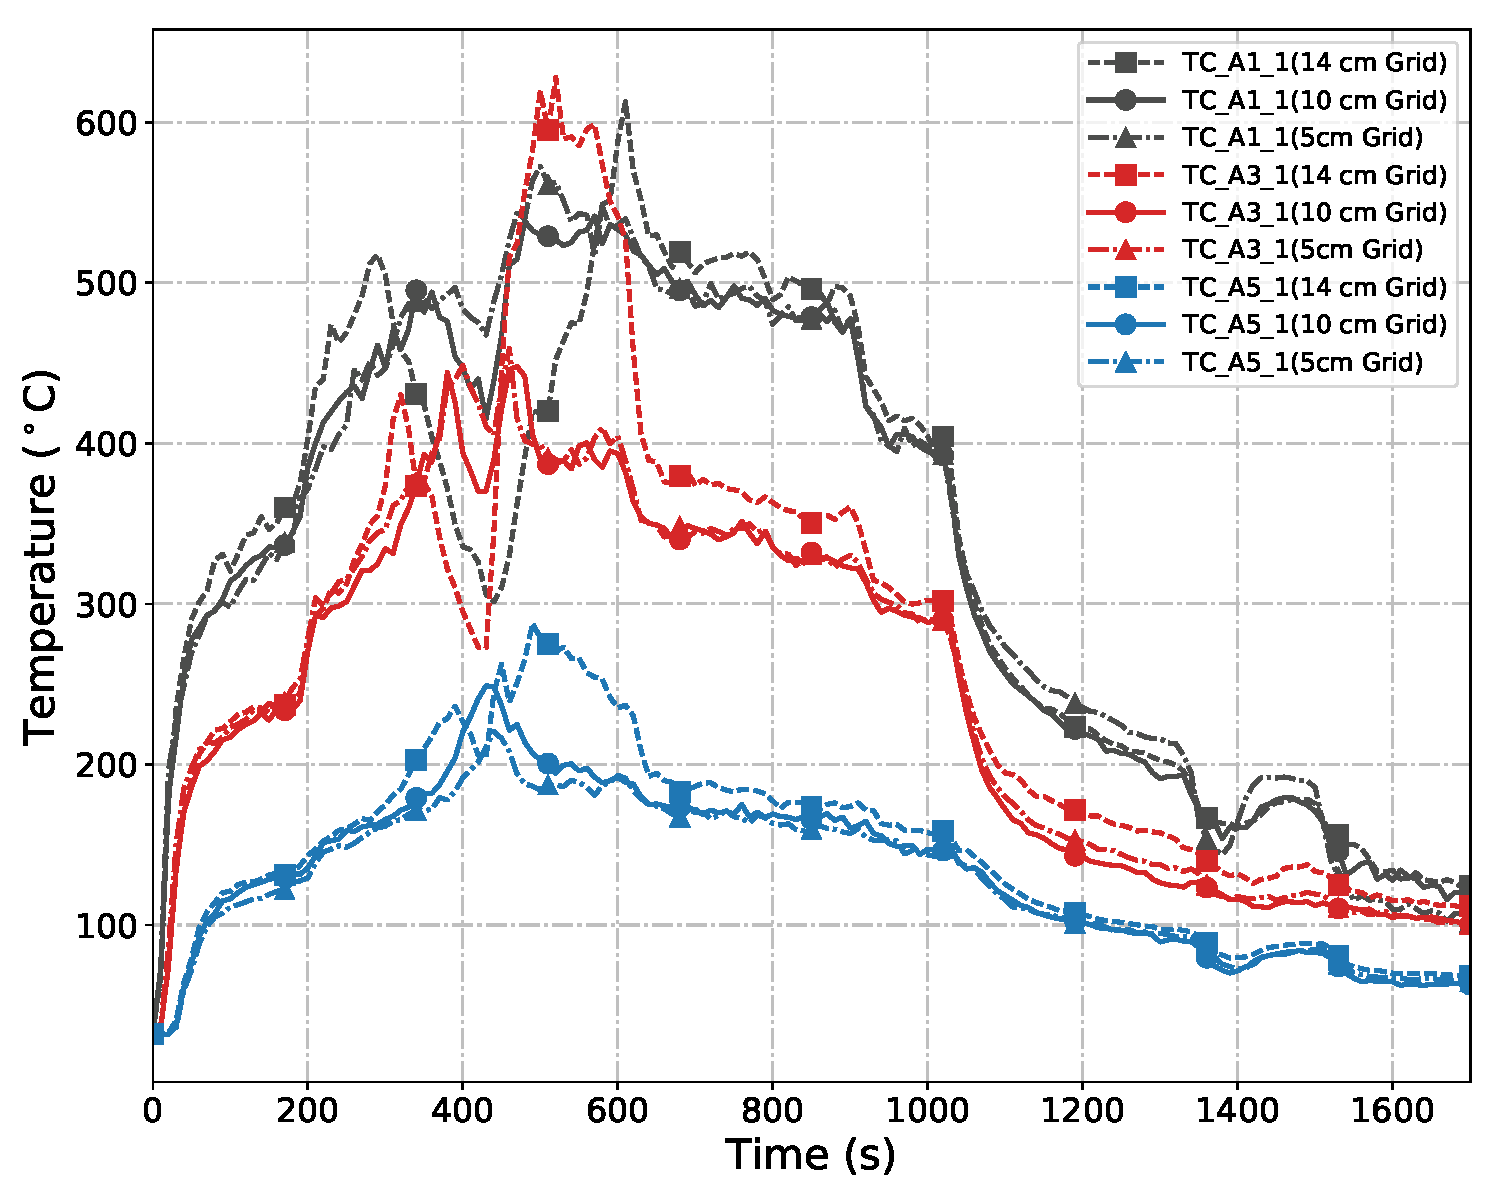
\includegraphics[width=0.87\columnwidth]{Figures/Plots/Grid_Sensitivity/Temperature/Test_04_cjet_1}
	\\~\\
	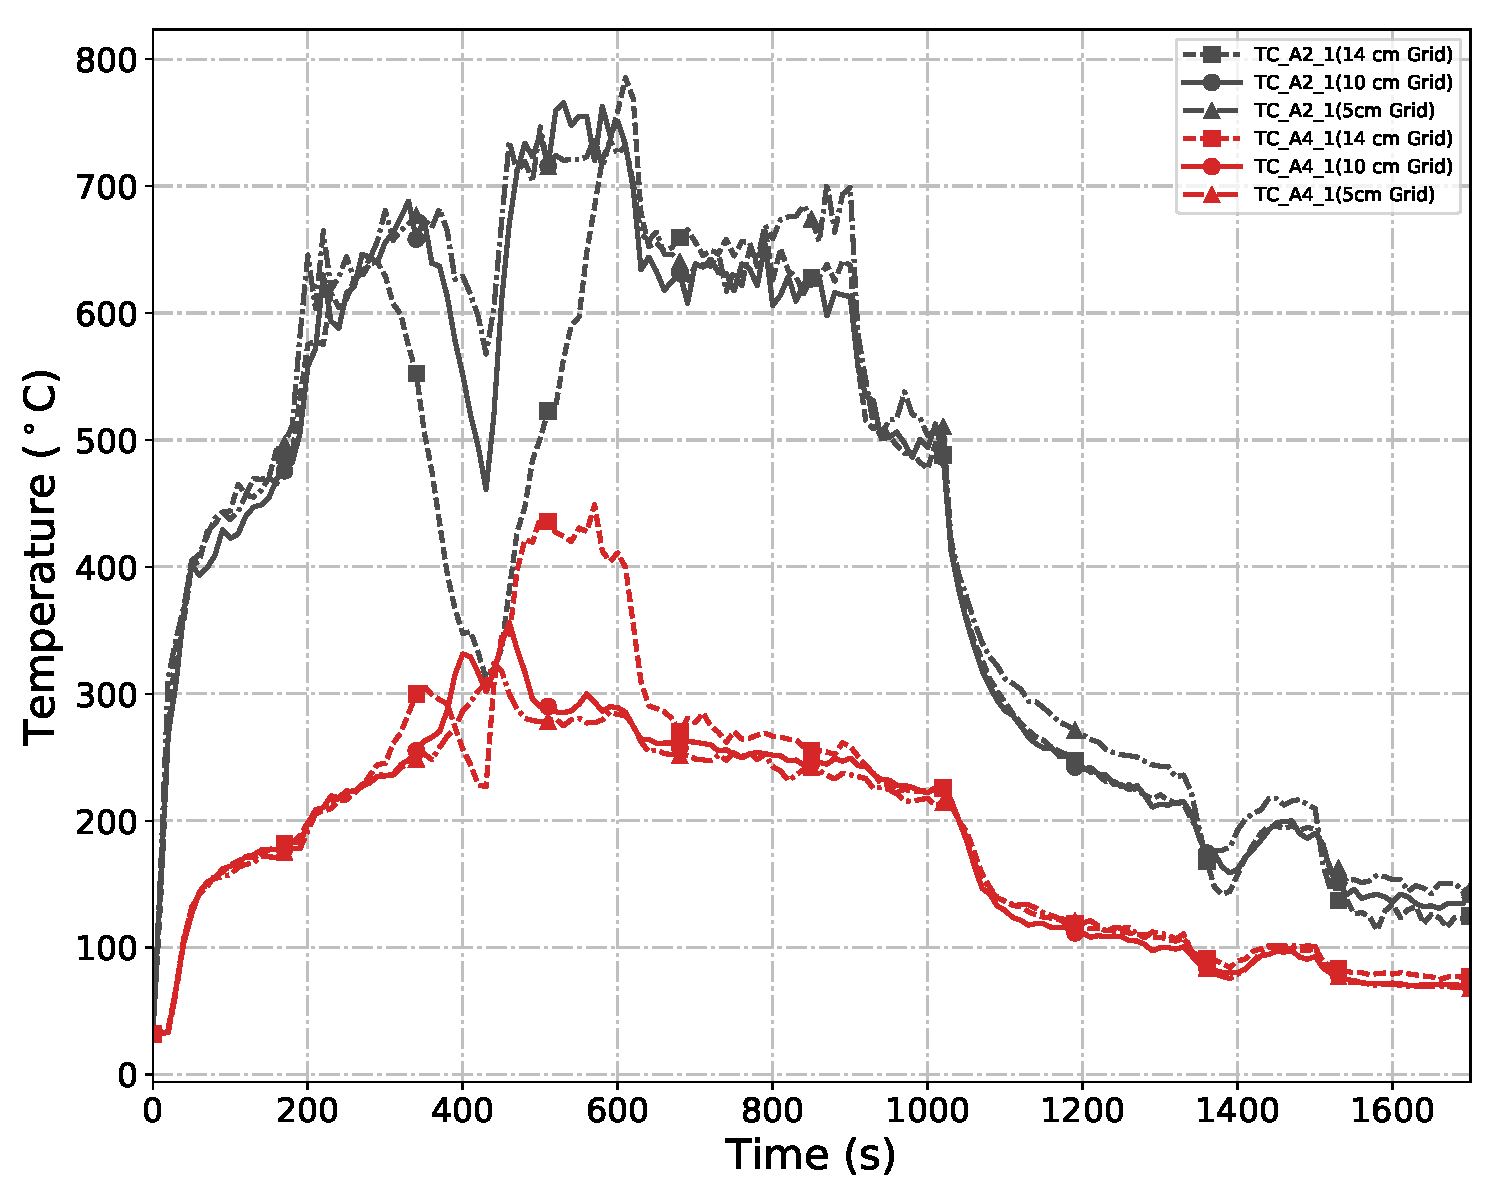
\includegraphics[width=0.87\columnwidth]{Figures/Plots/Grid_Sensitivity/Temperature/Test_04_cjet_2}
	\caption[Ceiling jet temperatures for East Structure simulation with different grid cell sizes.]{Ceiling jet temperatures output by the FDS simulation of Test~4 in the East Structure using three different grid cell sizes.}
	\label{fig:east_cjet_sensitivity}
\end{figure}

\begin{figure}[!h]
	\centering
	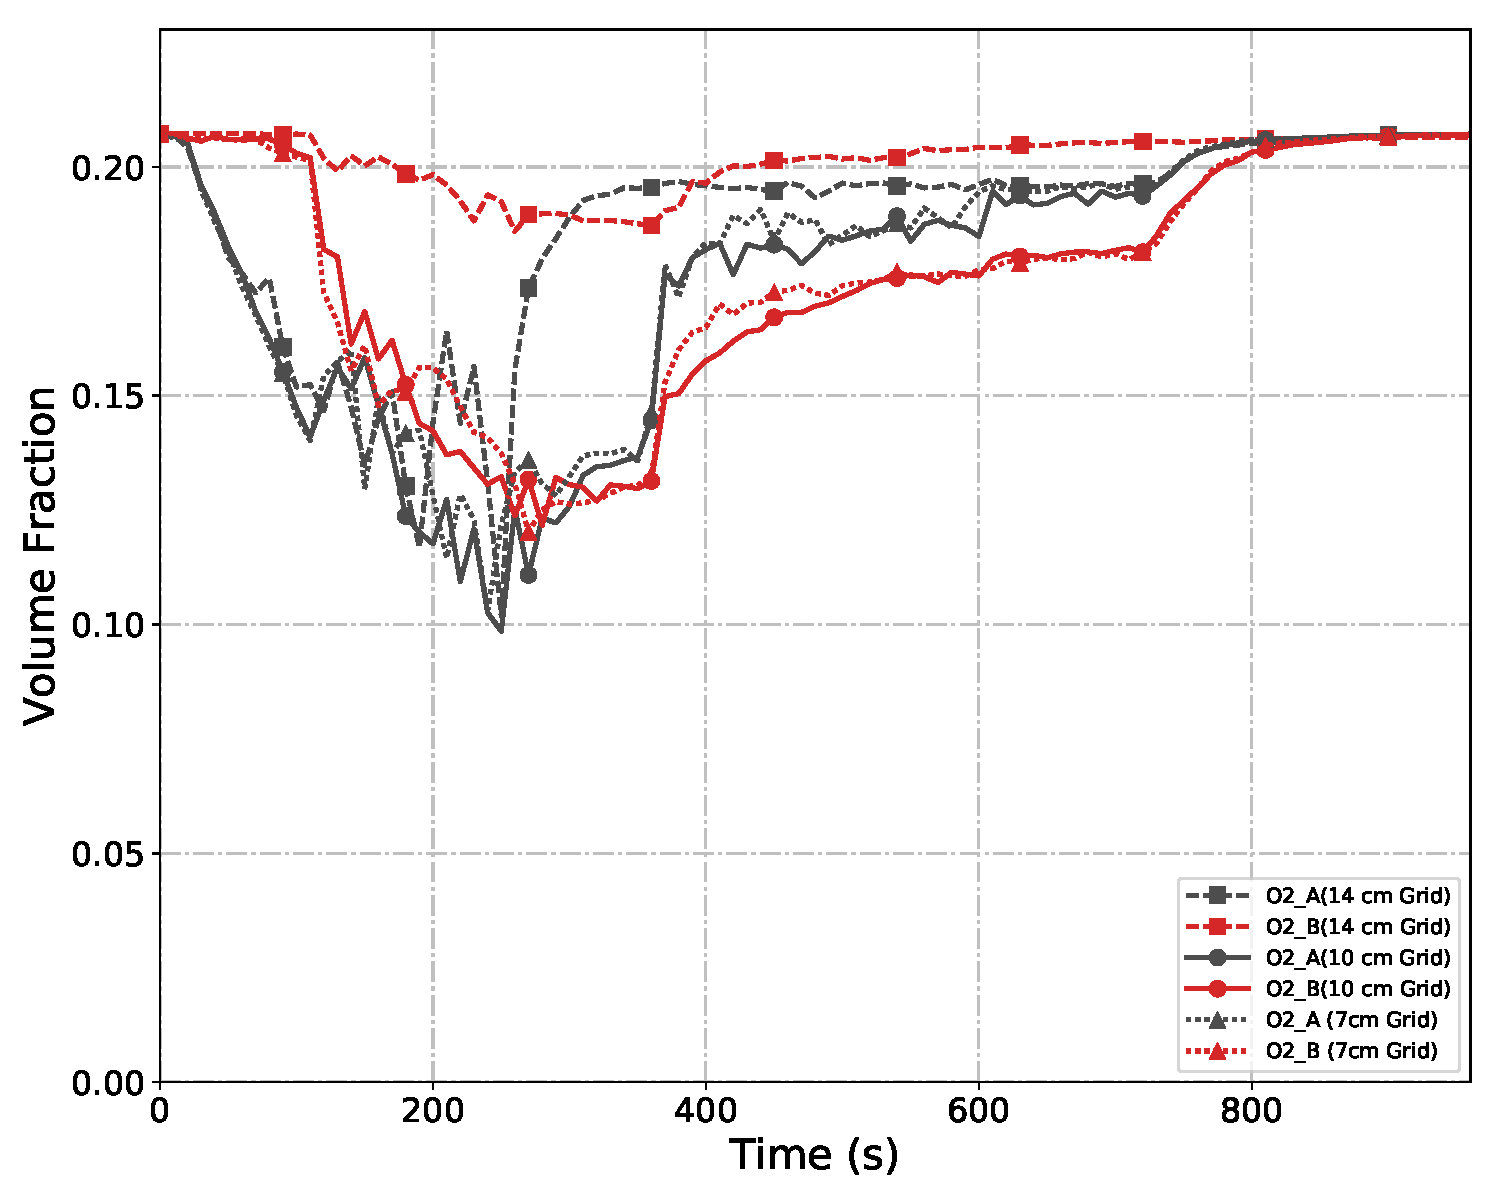
\includegraphics[width=\columnwidth]{Figures/Plots/Grid_Sensitivity/Gas_Concentration/Test_25_O2}
	\caption[$O_2$ concentrations for West Structure simulation with different grid cell sizes.]{$O_2$ concentrations output by the FDS simulation of Test~25 in the West Structure using three different grid cell sizes.}
	\label{fig:west_O2_sensitivity}
\end{figure}

\begin{figure}[!h]
	\centering
	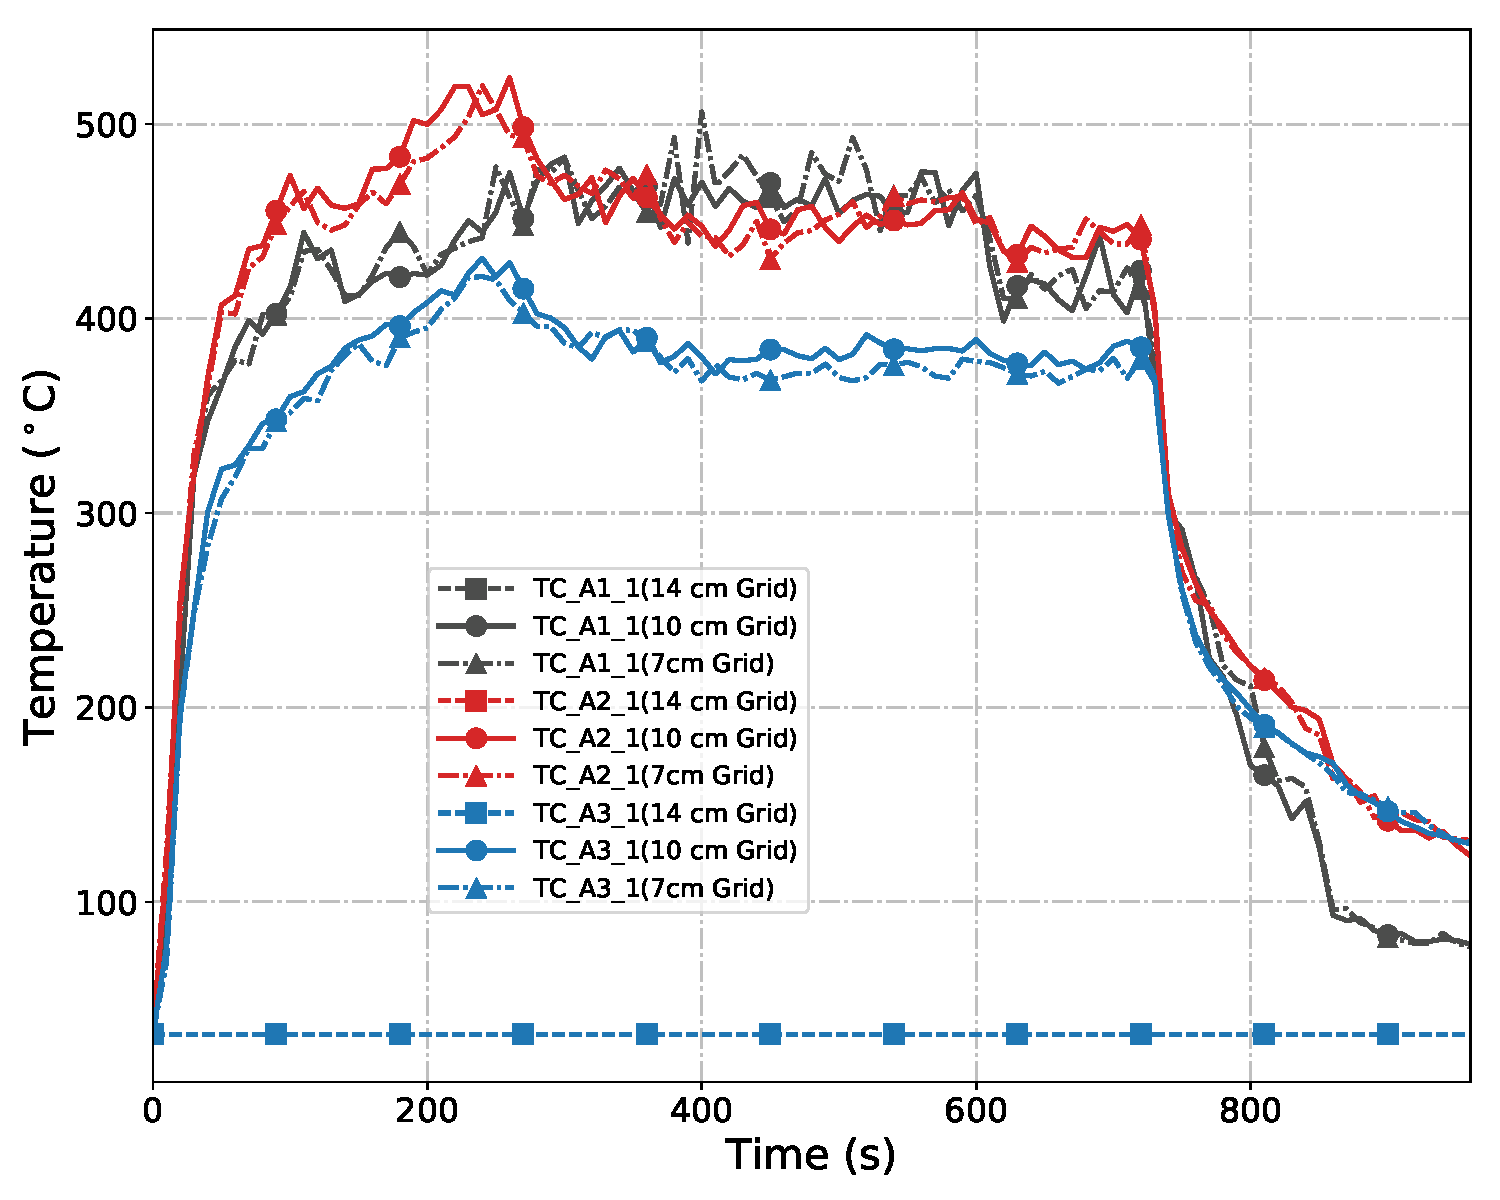
\includegraphics[width=0.87\columnwidth]{Figures/Plots/Grid_Sensitivity/Temperature/Test_25_cjet_1}
	\\~\\
	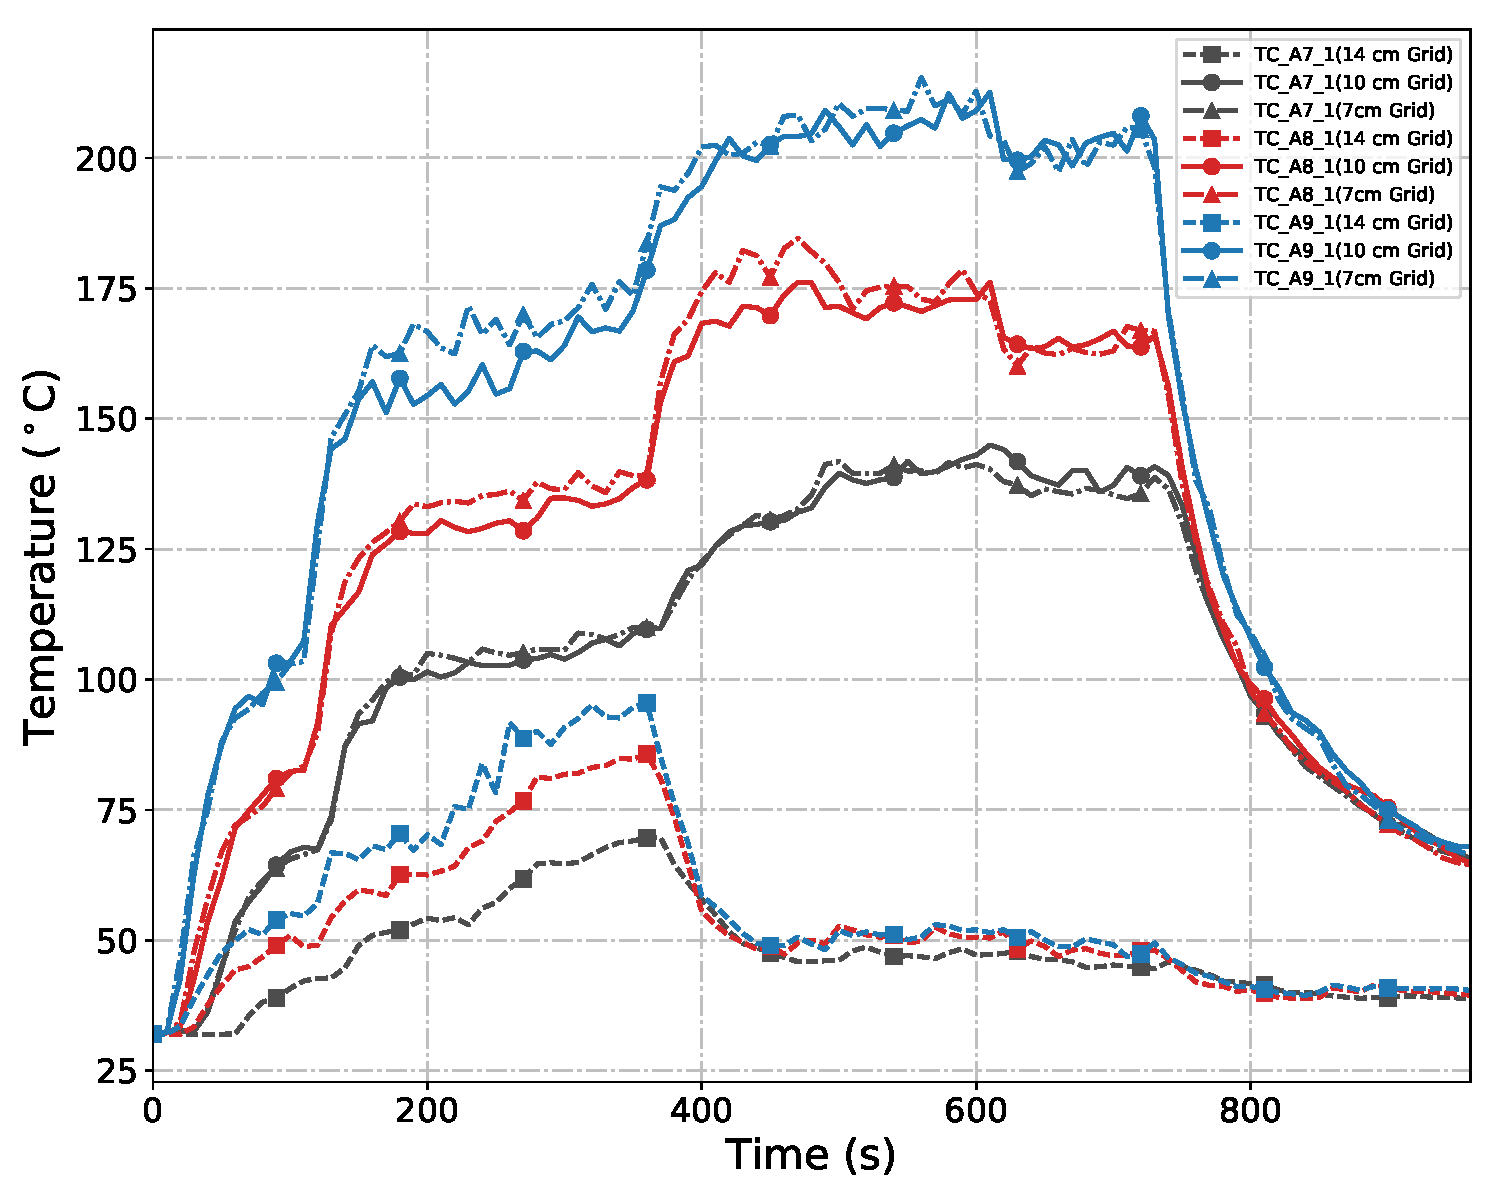
\includegraphics[width=0.87\columnwidth]{Figures/Plots/Grid_Sensitivity/Temperature/Test_25_cjet_2}
	\caption[Ceiling jet temperatures for West Structure simulation with different grid cell sizes.]{Ceiling jet temperatures output by the FDS simulation of Test~25 in the West Structure using three different grid cell sizes.}
	\label{fig:west_cjet_sensitivity}
\end{figure}

\FloatBarrier

The plots presented above show that significant differences occur at various times between the model data produced using the coarse grid and the same model data produced using the medium and fine grid resolutions. For example, looking at Figure~\ref{fig:west_O2_sensitivity}, the oxygen volume fraction data on the first floor of the West Structure output by the coarse grid deviates significantly from the data produced by medium and fine grid sizes around 300 seconds. Furthermore, the oxygen volume fraction data on the second floor output using the coarse grid drops to a minimum of approximately 0.18 during the portion of the simulation in which the burners are ignited, while the volume fraction data output using the medium and fine grids drop to a similar minimum that is around 0.13. 

Looking at the oxygen volume fraction and ceiling jet temperature data output by the East Structure simulation, Figures~\ref{fig:east_O2_sensitivity} and \ref{fig:east_cjet_sensitivity}, respectively, for different mesh resolutions, the data from the coarse grid exhibits more agreement with the medium and fine grid data than the West Structure simulation data plots. However, significant differences still arise between the coarse grid data and the simulation data produced by the medium and fine resolutions, such as the larger decline in ceiling jet temperature seen around 400~seconds.   

% Notice in Figure~\ref{fig:west_cjet_sensitivity}, the 14~cm grid was not refined enough to define the thermocouple locations at 0.03~m below the ceiling. 
Due to the large discrepancies between the coarse grid data and the data produced by the other two mesh resolutions, the coarse grid was considered too coarse for all simulations of the burner experiments. However, there doesn't appear to be any significant differences between the simulation data produced by the medium mesh resolution and the simulation data produced by the fine mesh resolution. As a result, the medium grid cell size of 10~cm was selected for all nine FDS simulations.

\section{FDS Model Data Compared to Experimental Data}
In the following subsections, the temperature, gas species concentration, gas velocity, and heat flux measurements predicted by the FDS simulations are compared to the corresponding sensor data measured during the propane burner experiments. Two different types of graphs are included to aid in the comparison of the model data and experimental data. The first type is similar to the mesh sensitivity study figures in that it shows the simulation data and experimental data (time-averaged over 10~seconds) plotted over the duration of an experiment for a specific data type at a specific location(s). Only one plot is presented for each discussed data quantity; the remaining figures of the discussed data types plotted over the duration each experiment for the different measurement locations are included in Appendix~\ref{chap:exp_FDS_plots}.

The second type of figure presented with each data quantity discussion summarizes the model uncertainty in predicting the specific data quantity. The summary graphs are similar to those presented in the FDS Validation Guide~\cite{FDS_Validation_Guide} --- each is a log/log scatter plot in which the $x$ value of each point is based on a set of measured, experimental data and the $y$ value of each point is based on the equivalent set of predicted data from the FDS simulation. No data from Tests~2--4 were used to generate the summary scatter plots because the heat release rates prescribed to the FDS simulations of the tests were determined through the use of a correlation (MQH) based on the experimental temperature data instead of through a direct physical measurement, such as the flow rate of propane to the burners used to determine the prescribed heat release rates for the other six simulations. The procedure used to generate the scatter plots and statistical data is briefly outlined below. Full details of the analysis are described in detail in by McGrattan and Toman in Ref.~\cite{McGrattan:Metrologia}.

Taking $M_i$ and $E_i$ to represent the change in the value of a quantity from its ambient at a specific time based on the data output by the FDS simulation and measured by instrumentation during the experiment, respectively, the mean and standard deviation of the distribution can be estimated by first calculating
\begin{equation} 
	\overline{\ln(M/E)}=\frac{1}{n} \sum_{i=1}^n \ln\left( \frac{M_i}{E_i} \right)
\end{equation}
Note, the natural logarithm function is used so that the variance of the random variable can be expressed in terms of the relative uncertainty. The assumption that $\ln(M/E)$ is normally distributed has been tested for each data type of interest by the developers of FDS, and the results are shown in the FDS Validation Guide. The standard deviation of the logarithm of a normally distributed random variable is approximately equal to the standard deviation divided by its mean, the relative standard deviation. The least squares estimate of the standard deviation of the combined distribution is defined as:
\begin{equation}
\label{eq:least_sqrs}
	\widetilde{\sigma}_m^2 + \widetilde{\sigma}_E^2 \approx \frac{1}{n-1}\sum_{i=1}^n \left[ \ln(M_i/E_i) - \overline{\ln(M/E)} \right]^2
\end{equation}
Using the pair of measured and predicted values with the known $\widetilde{\sigma}_E$, the expression on the right can be evaluated. Eq.~\ref{eq:least_sqrs} imposes a constraint on the experimental uncertainty value, $\widetilde{\sigma}_E$, and in combination with a second constraint that $\widetilde{\sigma}_M$ cannot be less than $\widetilde{\sigma}_E$ because it's impossible to show that the model is more accurate than the measurements against which it's compared, the following is produced:
\begin{equation}
	\widetilde{\sigma}_E^2 \leq \frac{1}{2}\textrm{Var}(\ln(M/E))
\end{equation}
Using the mean of the distribution, an estimate of a bias factor, $\delta$, which expresses the tendency of the model to over or under-predict the measured quantity, can be found:
\begin{equation}
	\delta \approx \exp\left( \overline{\ln(M/E)}+\frac{\widetilde{\sigma}_M^2}{2}-\frac{\widetilde{\sigma}_E^2}{2} \right)
\end{equation}

The values of $\delta$, $\sigma_M$, and $\sigma_E$ are reported with each log/log plot in the following sections. For each plot, the solid red line and solid black line represent the expected values for $M$ and $E$, respectively, and the dashed lines represent $\pm \sigma$, or standard deviations, of the data corresponding to the line color. Each plotted gray point represents an average value of the specific data quantity across a 30 second test period in which one or more gas burners were ignited and only natural ventilation was present throughout the structure (i.e., no PPV fan was turned on). All the points are based on computed values over the applicable time periods of Tests~5--6 and Tests~22--25. Table~\ref{table:stats_compare} in the final section of this chapter summarizes the statistical values calculated for each data type and is presented with a brief discussion of how the values compare to the same statistical values listed in the FDS Validation Guide.

\subsection{Temperature}

\subsubsection*{\textit{Hot Gas Layer}}
A quantity that is commonly estimated for compartment fire scenarios is the location of the interface between the hot, smoke-laden upper layer and cooler, lower layer. Some fire models, such as two-zone models, calculate this value directly, along with the average temperature of the upper (hot gas) layer and lower layer. Being that it's a CFD model, FDS computes a continuous profile of temperature and thus, does not directly calculate the interface location or the average temperature of each layer. However, numerous techniques exist to estimate the layer height and average temperatures from a continuous vertical profile of temperature. The temperatures measured by the thermocouples in the vertical arrays throughout the experimental structures were used to define a vertical profile of temperature, $T(z)$, in which $z$ is the height above the floor ($z=0$ at the floor and $z=H$ at the room's ceiling). Then, the vertical temperature profile was used to estimate the hot gas layer temperature by a method developed by Janssens and Tran~\cite{Janssens:JFS1992}. Taking $T_u$ as the upper layer temperature, $T_l$ as the lower layer temperature, and $z_{int}$ as the hot gas layer interface height, the method is outlined below, starting with the calculation of the quantities $I_1$ and $I_2$
\begin{equation*}
	I_1 = \int^H_0 T(z)dz = (H-z_{int})T_u+z_{int}T_l
\end{equation*}
\begin{equation*}
	I_2 = \int^H_0 \frac{1}{T(z)}dz = (H-z_{int})\frac{1}{T_u}+z_{int}\frac{1}{T_l}
\end{equation*}
$I_1$ and $I_2$ are then used to solve for $z_{int}$ as follows
\begin{equation}
	z_{int}=\frac{T_l(I_1I_2-H^2)}{I_1+I_2 T_l^2-2T_l H}
\end{equation}
$T_l$ is the temperature in the lowest mesh cell (or thermocouple) and $T_u$ is the average upper layer temperature defined by
\begin{equation}
	(H-z_{int})T_u=\int^H_{z_{int}} T(z)dz
\end{equation}

Figure~\ref{fig:HGL_data} shows the hot gas layer temperature derived from experimental data plotted with the same quantity derived from the FDS simulation data for Test~22, and Figure~\ref{fig:loglog_HGL} shows the log/log scatter plot of the hot gas layer temperatures obtained from the predicted data from the FDS simulations compared to the values obtained by the measured data for the six applicable gas burner experiments. 

\begin{figure}[!h]
	\centering
	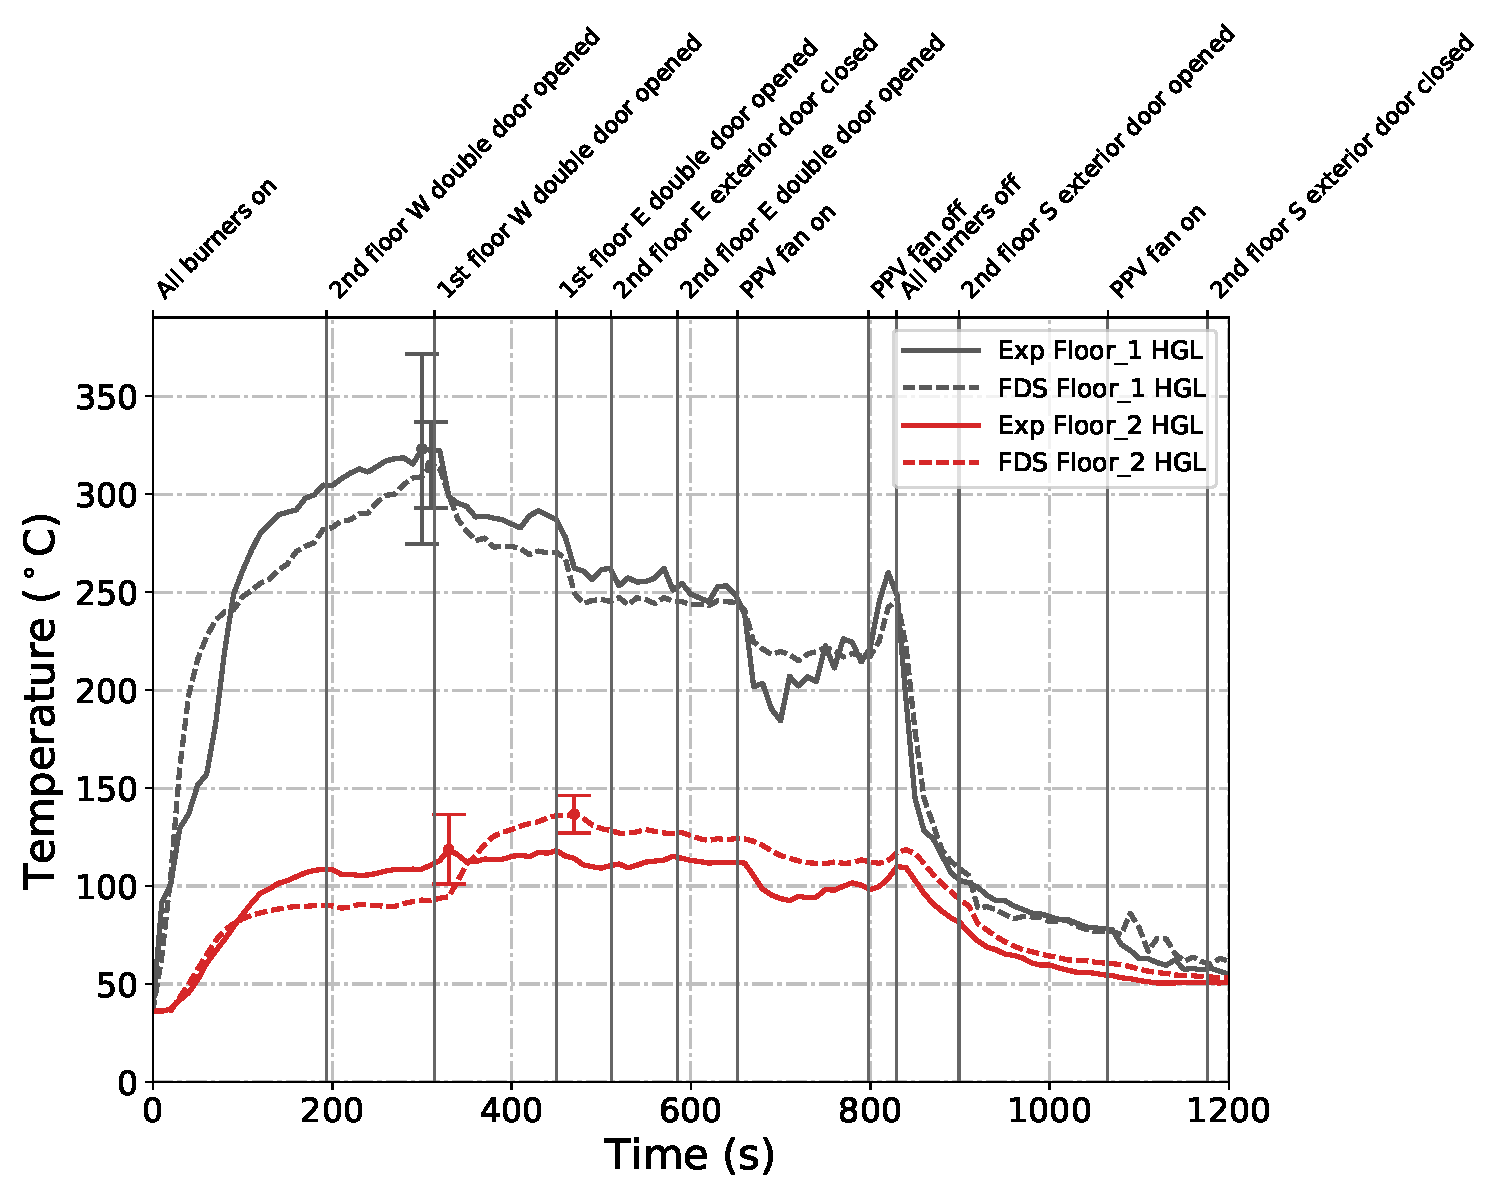
\includegraphics[width=\columnwidth]{Figures/Plots/Validation/Temperature/Test_22_HGL}
	\caption[Plots of measured and predicted hot gas layer temperatures during Test~22.]{Plots of measured and predicted hot gas layer temperatures on the first and second floors of the West Structure during Test~22.}
	\label{fig:HGL_data}
\end{figure}

\begin{figure}[!h]
	\centering
	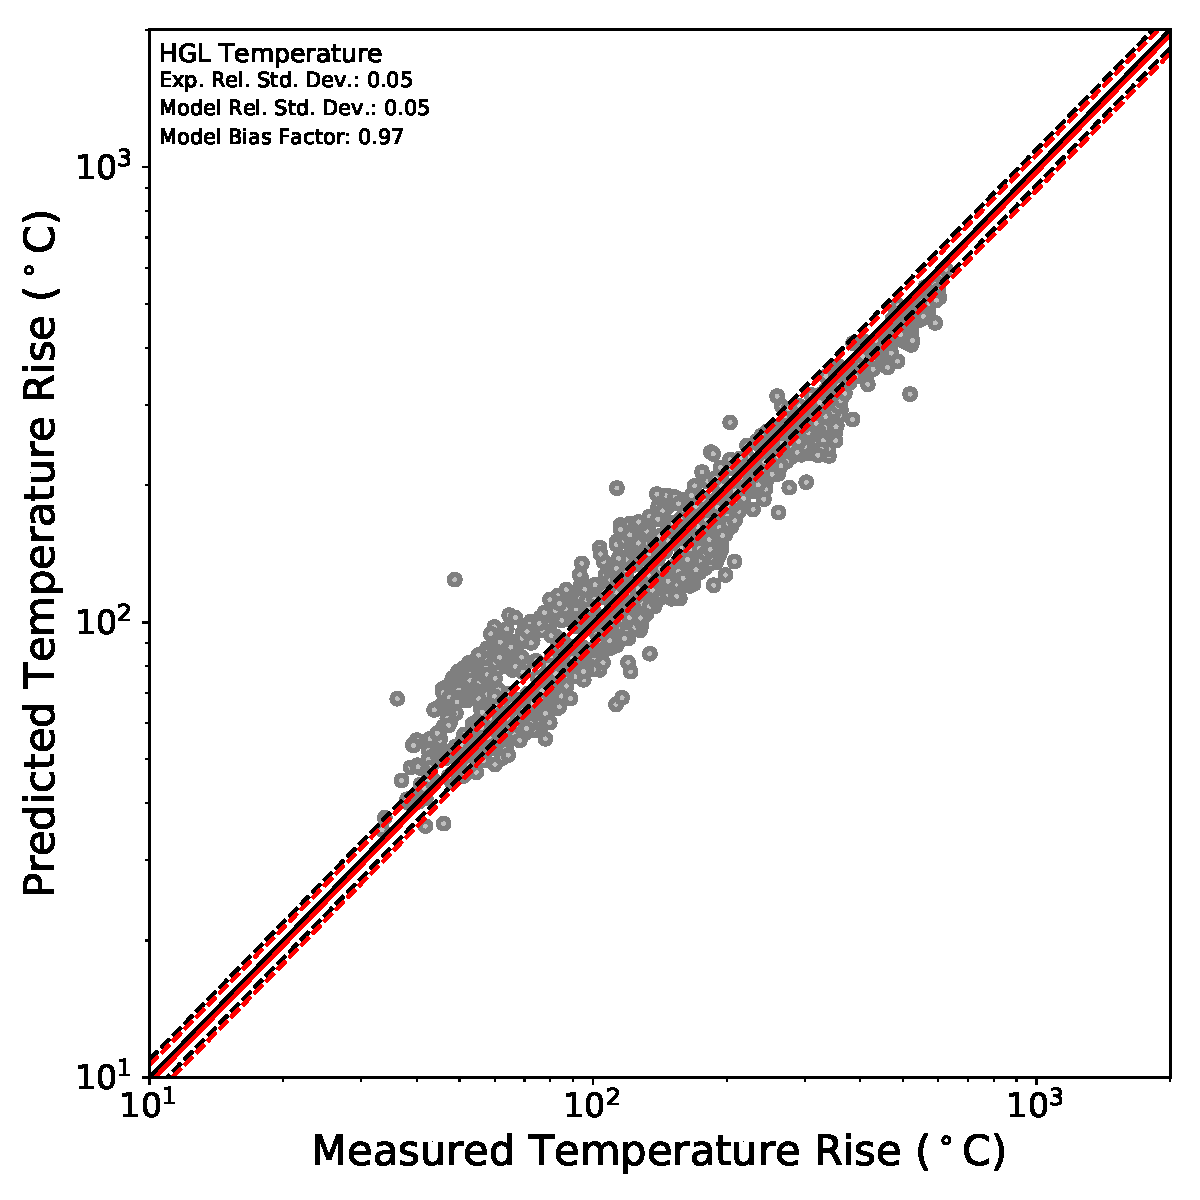
\includegraphics[width=\columnwidth]{Figures/Plots/Validation/Temperature/loglog_HGL}
	\caption{Summary of measured and predicted hot gas layer temperatures.}
	\label{fig:loglog_HGL}
\end{figure}

\FloatBarrier
\subsubsection*{\textit{Ceiling Jet}}
The temperature near the ceiling can be a used to evaluate a model's ability to predict the activation times of sprinklers, smoke detectors, and other fire protection devices at ceiling height. The ``ceiling jet'' temperature used throughout this report refers to the temperature measured by the top thermocouple (closest to the ceiling) of the various thermocouple arrays located throughout the experimental structures. Figure~\ref{fig:cjet_data} shows the ceiling jet temperatures measured during Test~4 plotted with the ceiling jet temperatures predicted by the FDS model for the same duration. Figure~\ref{fig:loglog_cjets} shows the log/log scatter plot of the ceiling jet temperatures predicted by the FDS simulations compared to the corresponding measured ceiling jet temperatures for the six applicable gas burner experiments.
\begin{figure}[!h]
	\centering
	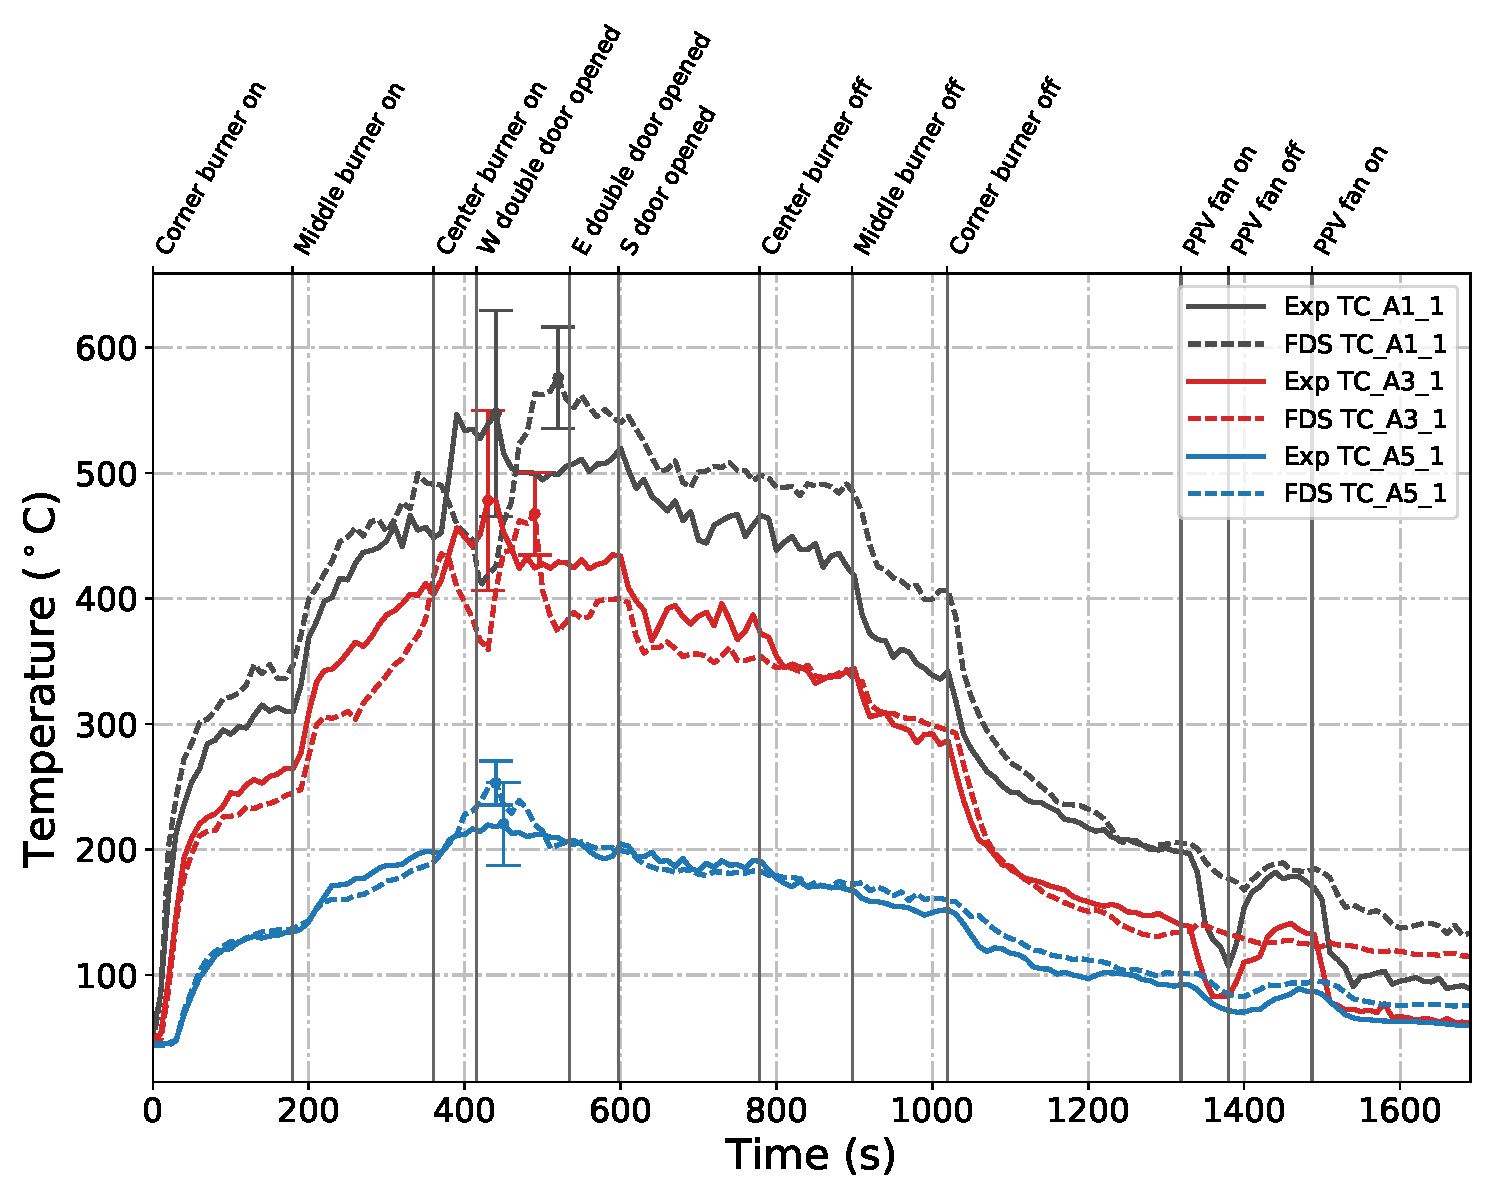
\includegraphics[width=\columnwidth]{Figures/Plots/Validation/Temperature/Test_4_cjet_1}
	\caption[Plots of measured and predicted ceiling jet temperatures during Test~4.]{Plots of measured and predicted ceiling jet temperatures during Test~4 obtained from thermocouple arrays A1, A3, and A5 located in the fire room, middle room, and north room, respectively.}
	\label{fig:cjet_data}
\end{figure}

\begin{figure}[!h]
	\centering
	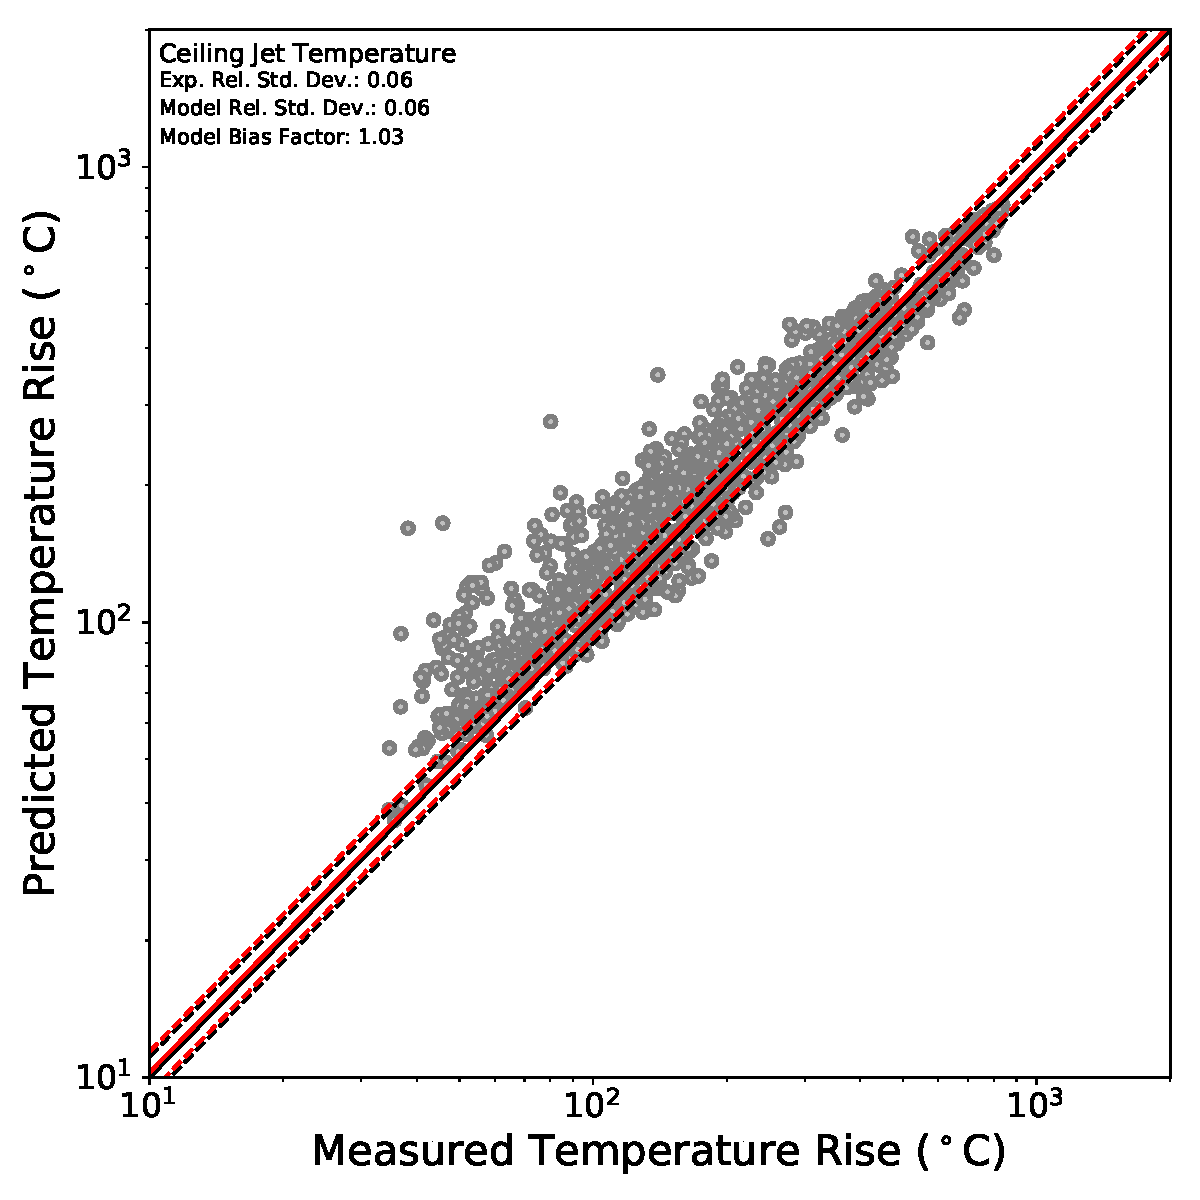
\includegraphics[width=\columnwidth]{Figures/Plots/Validation/Temperature/loglog_cjetTCs}
	\caption{Summary of measured and predicted ceiling jet temperatures.}
	\label{fig:loglog_cjets}
\end{figure}

\clearpage
\subsubsection*{\textit{Thermocouple Arrays}}
In addition to the hot gas layer and ceiling jet temperatures, the measured and predicted temperatures at each thermocouple location for each thermocouple array were compared. Two figures of the temperatures over the duration of each test were generated for each thermocouple array: one of the ``upper'' temperatures corresponding to the four thermocouple locations nearest to the ceiling and one of the ``lower'' temperatures corresponding to the four thermocouple locations nearest to the floor. Figure~\ref{fig:TCarray_data} contains the measured and predicted upper temperatures from array A1 over the duration of Test~24 and Figure~\ref{fig:loglog_TC_arrays} shows the log/log scatter plot of the temperatures measured at the different thermocouple locations within the thermocouple arrays compared to the temperatures at the same locations predicted by the FDS simulations for Tests~5--6 and Tests~22--25.
\begin{figure}[!h]
	\centering
	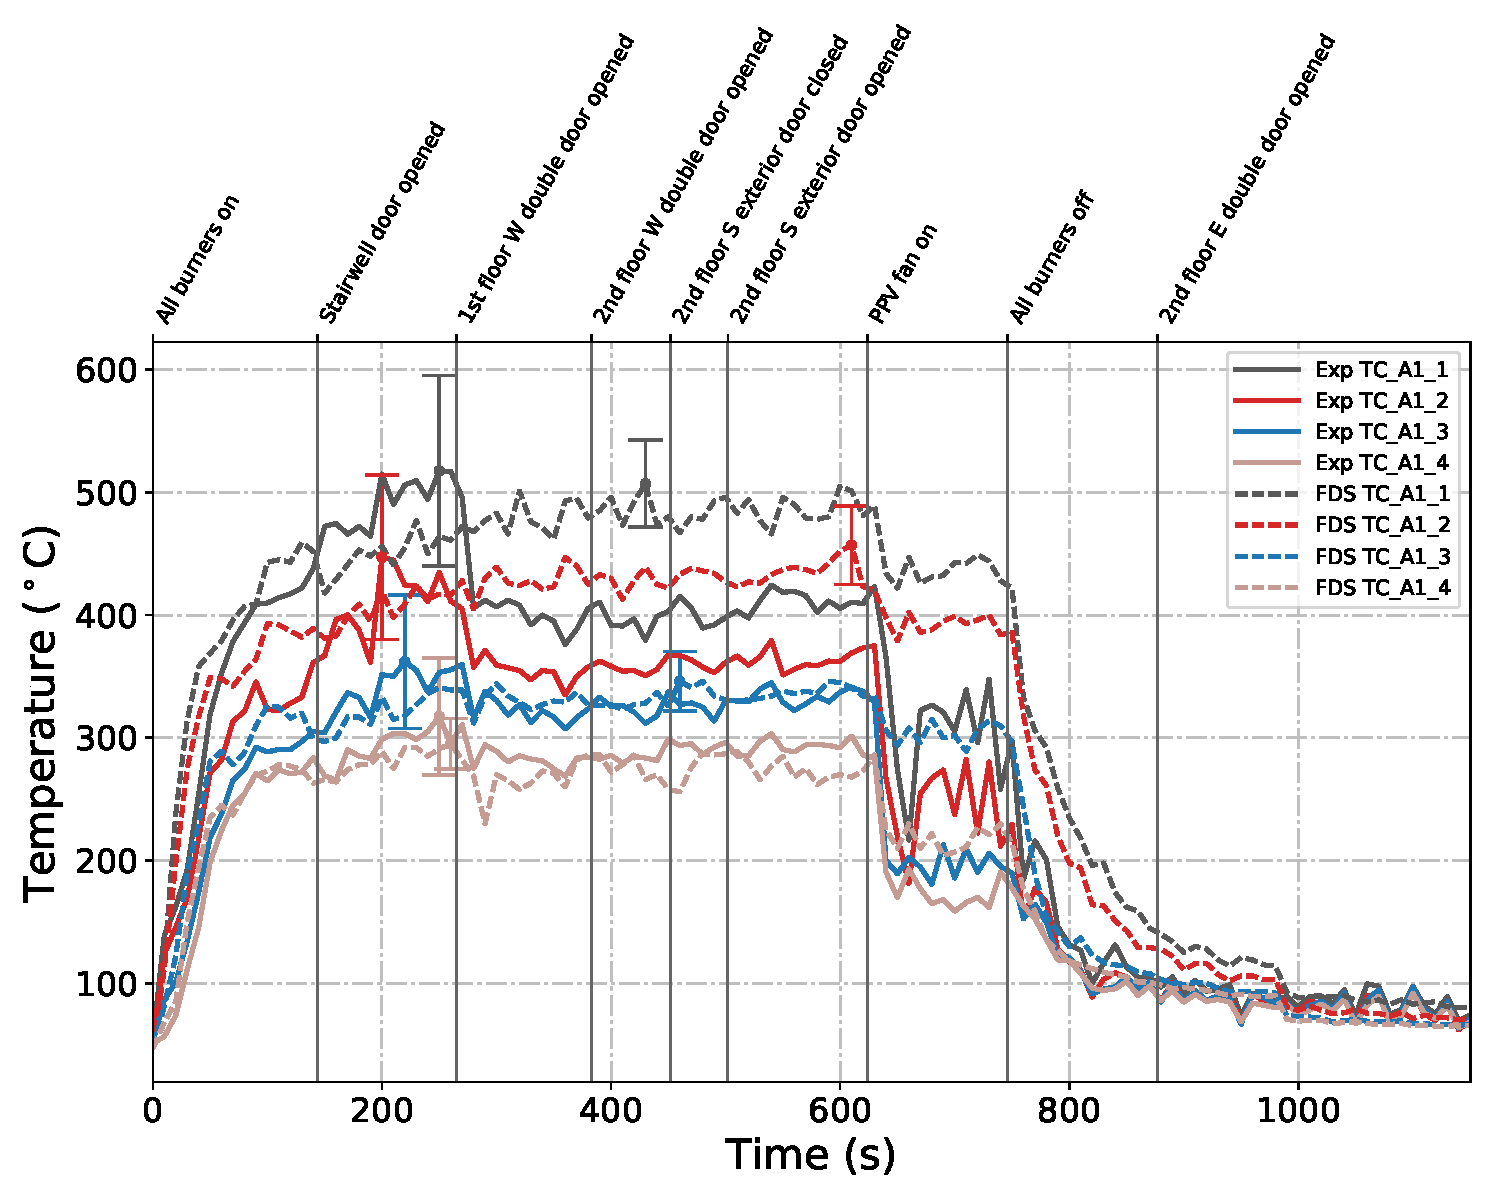
\includegraphics[width=\columnwidth]{Figures/Plots/Validation/Temperature/Test_24_TC_A1_upper}
	\caption[Plot of the measured and predicted upper temperatures from array A1 during Test~24.]{Plots of measured and predicted ``upper'' temperatures from array A1 during Test~24.}
	\label{fig:TCarray_data}
\end{figure}

\begin{figure}[!h]
	\centering
	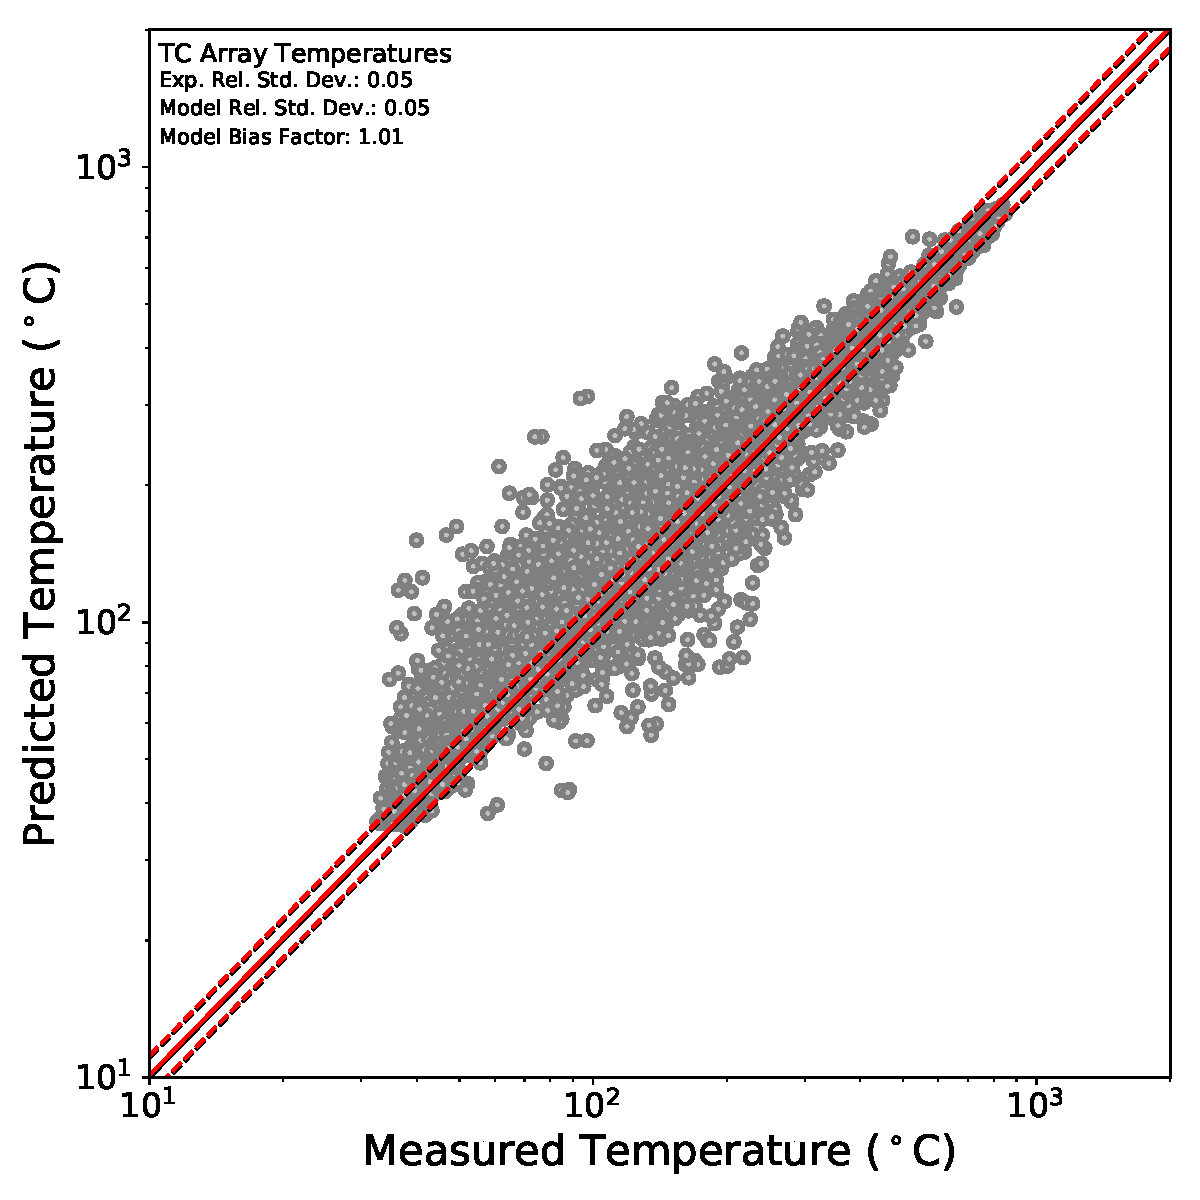
\includegraphics[width=\columnwidth]{Figures/Plots/Validation/Temperature/loglog_TC_arrays}
	\caption{Summary of measured and predicted temperatures at the individual thermocouple locations within the different thermocouple arrays.}
	\label{fig:loglog_TC_arrays}
\end{figure}

\clearpage
\subsection{Gas Species Concentration}

\subsubsection*{\textit{$O_2$} Concentration}
The measured and predicted oxygen concentrations of Room~1 (fire room) and Room~3 in the East Structure for the duration of Test~3 are shown in Figure~\ref{fig:Test3_O2} as the black and red plots, respectively. Additionally, the summary log/log scatter plot of the predicted oxygen concentrations compared to the corresponding measured oxygen concentrations for Tests~5--6 and Tests~22--25 is shown in Figure~\ref{fig:loglog_O2}.
\begin{figure}[!h]
	\centering
	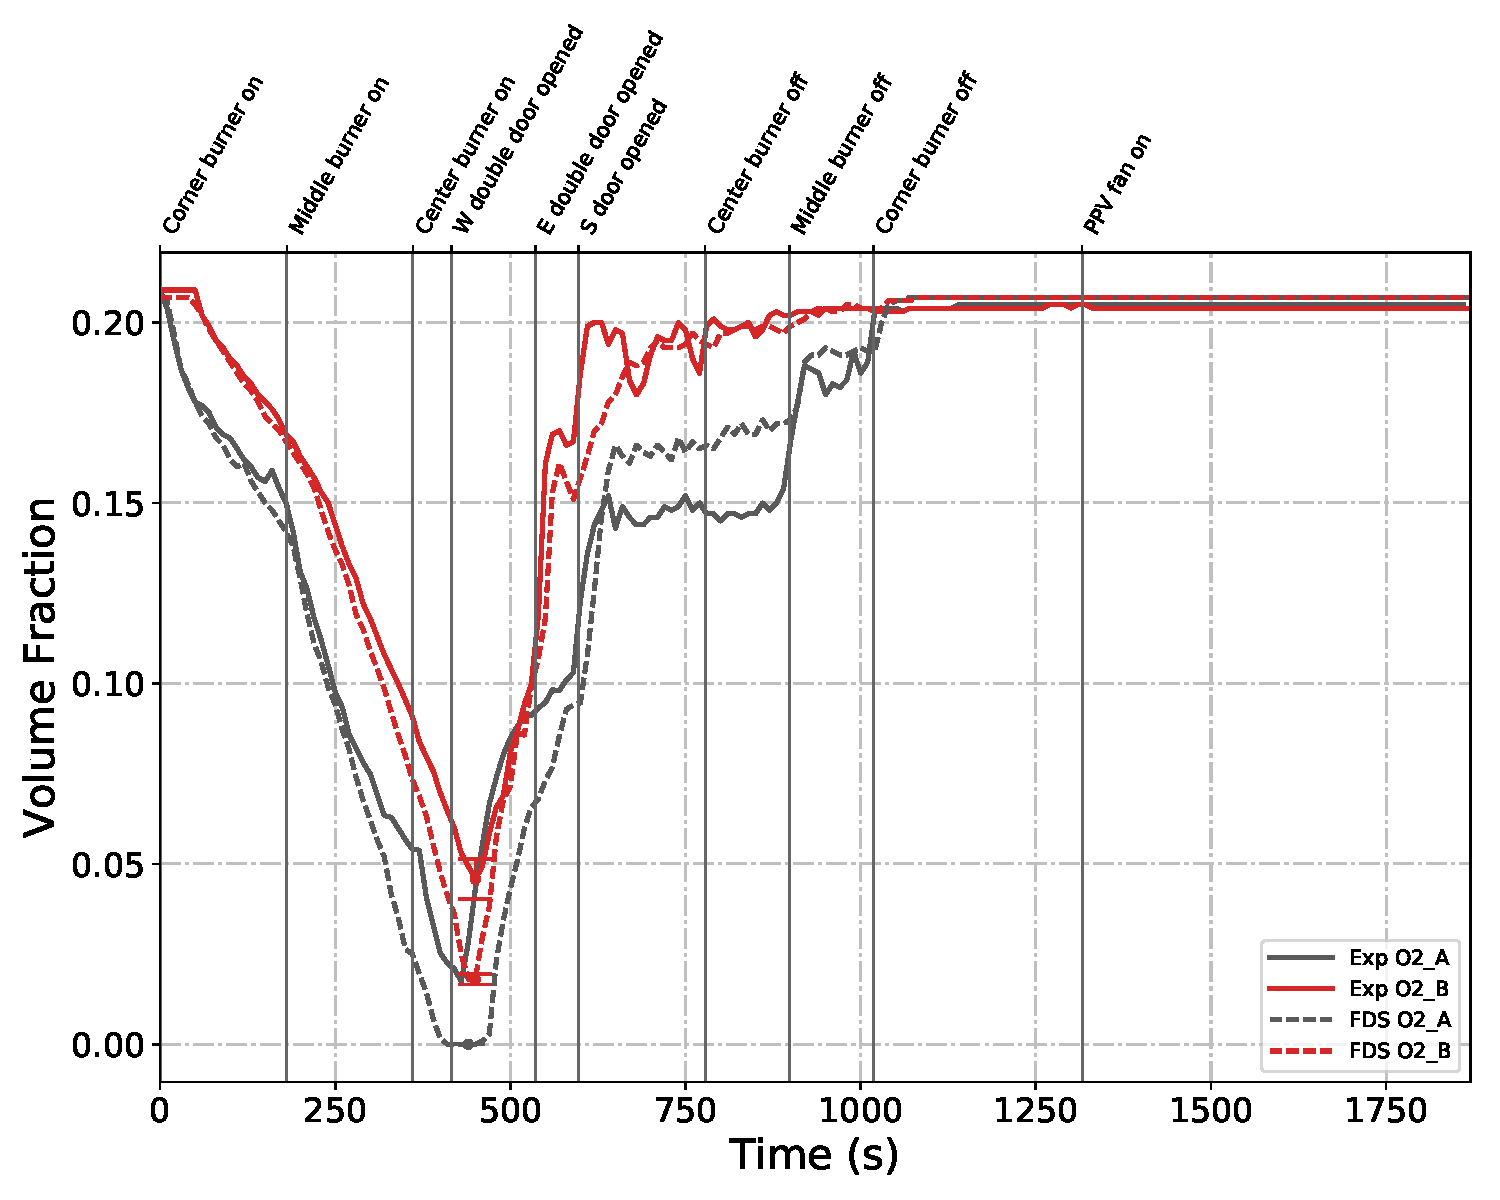
\includegraphics[width=\columnwidth]{Figures/Plots/Validation/Gas_Concentration/Test_3_O2}
	\caption[Plots of measured and predicted $O_2$ concentration during Test~3.]{Plots of measured and predicted $O_2$ concentration in the fire room (black plots) and north room (red plots) during Test~3.}
	\label{fig:Test3_O2}
\end{figure}

\begin{figure}[!h]
	\centering
	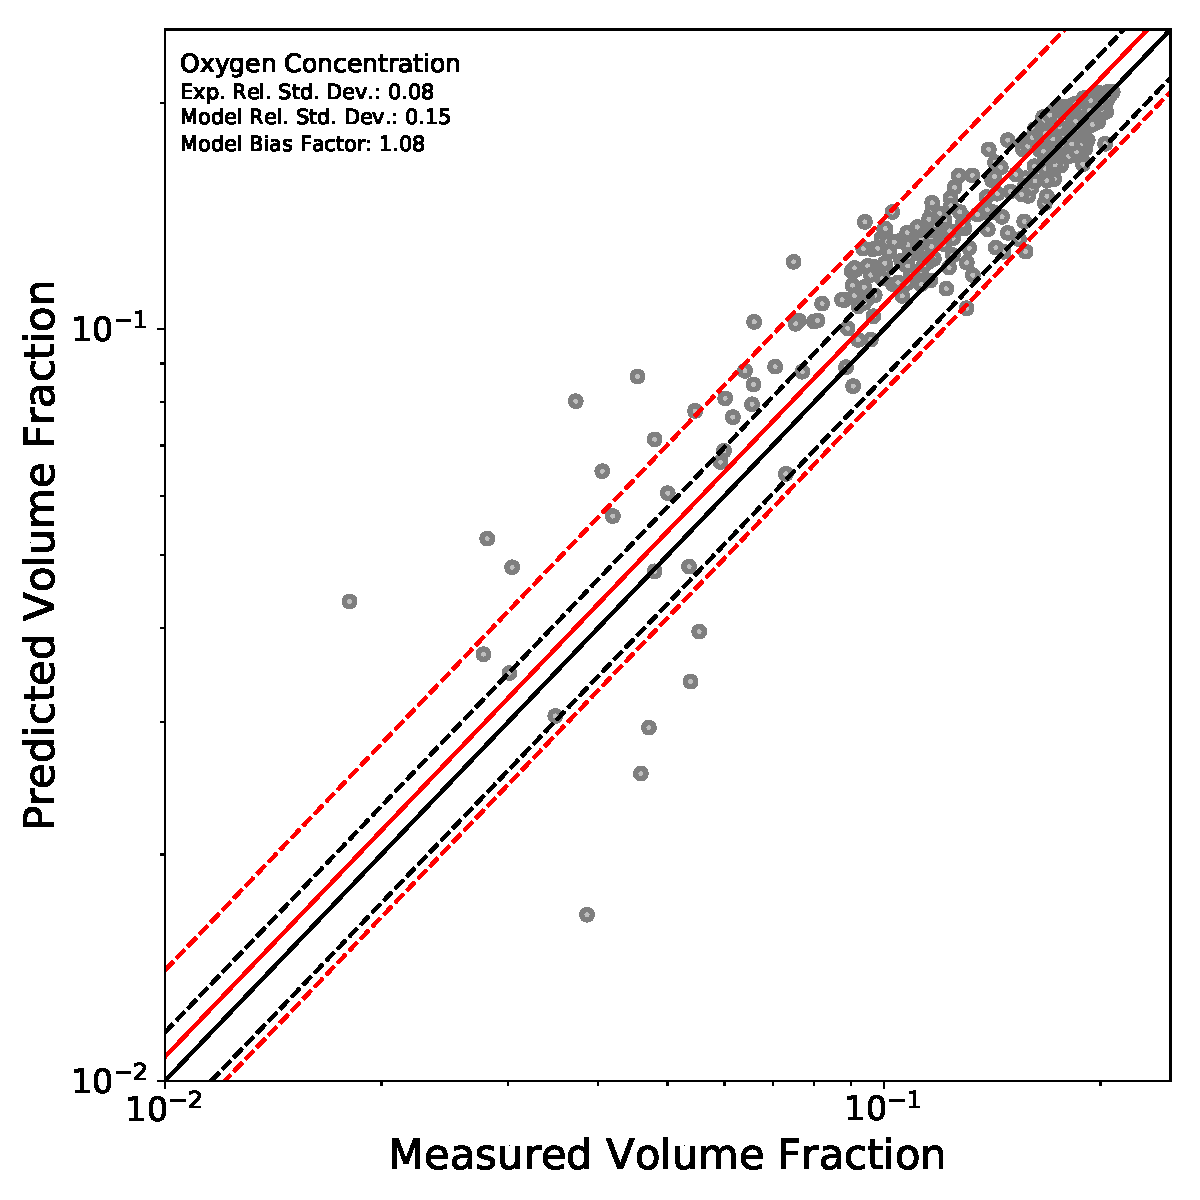
\includegraphics[width=\columnwidth]{Figures/Plots/Validation/Gas_Concentration/loglog_O2}
	\caption{Summary of measured and predicted $O_2$ concentrations.}
	\label{fig:loglog_O2}
\end{figure}

\FloatBarrier
\subsubsection*{\textit{$CO_2$} Concentration}
The measured and predicted carbon dioxide concentrations of Room~1 (fire room) and Room~3 in the East Structure for the duration of Test~3 are shown in Figure~\ref{fig:Test3_CO2} as the black and red plots, respectively. Note, the gas sampling system used to measure gas species concentrations could measure $CO_2$ concentrations below 0.10. Thus, data pairs from the applicable time ranges of Tests~5--6 and Tests~22--25 for which the measured $CO_2$ volume fraction was 0.10 were not used to create the summary log/log scatter plot of the predicted carbon dioxide concentrations compared to the corresponding measured carbon dioxide concentrations shown in Figure~\ref{fig:loglog_CO2} below.
\begin{figure}[!h]
	\centering
	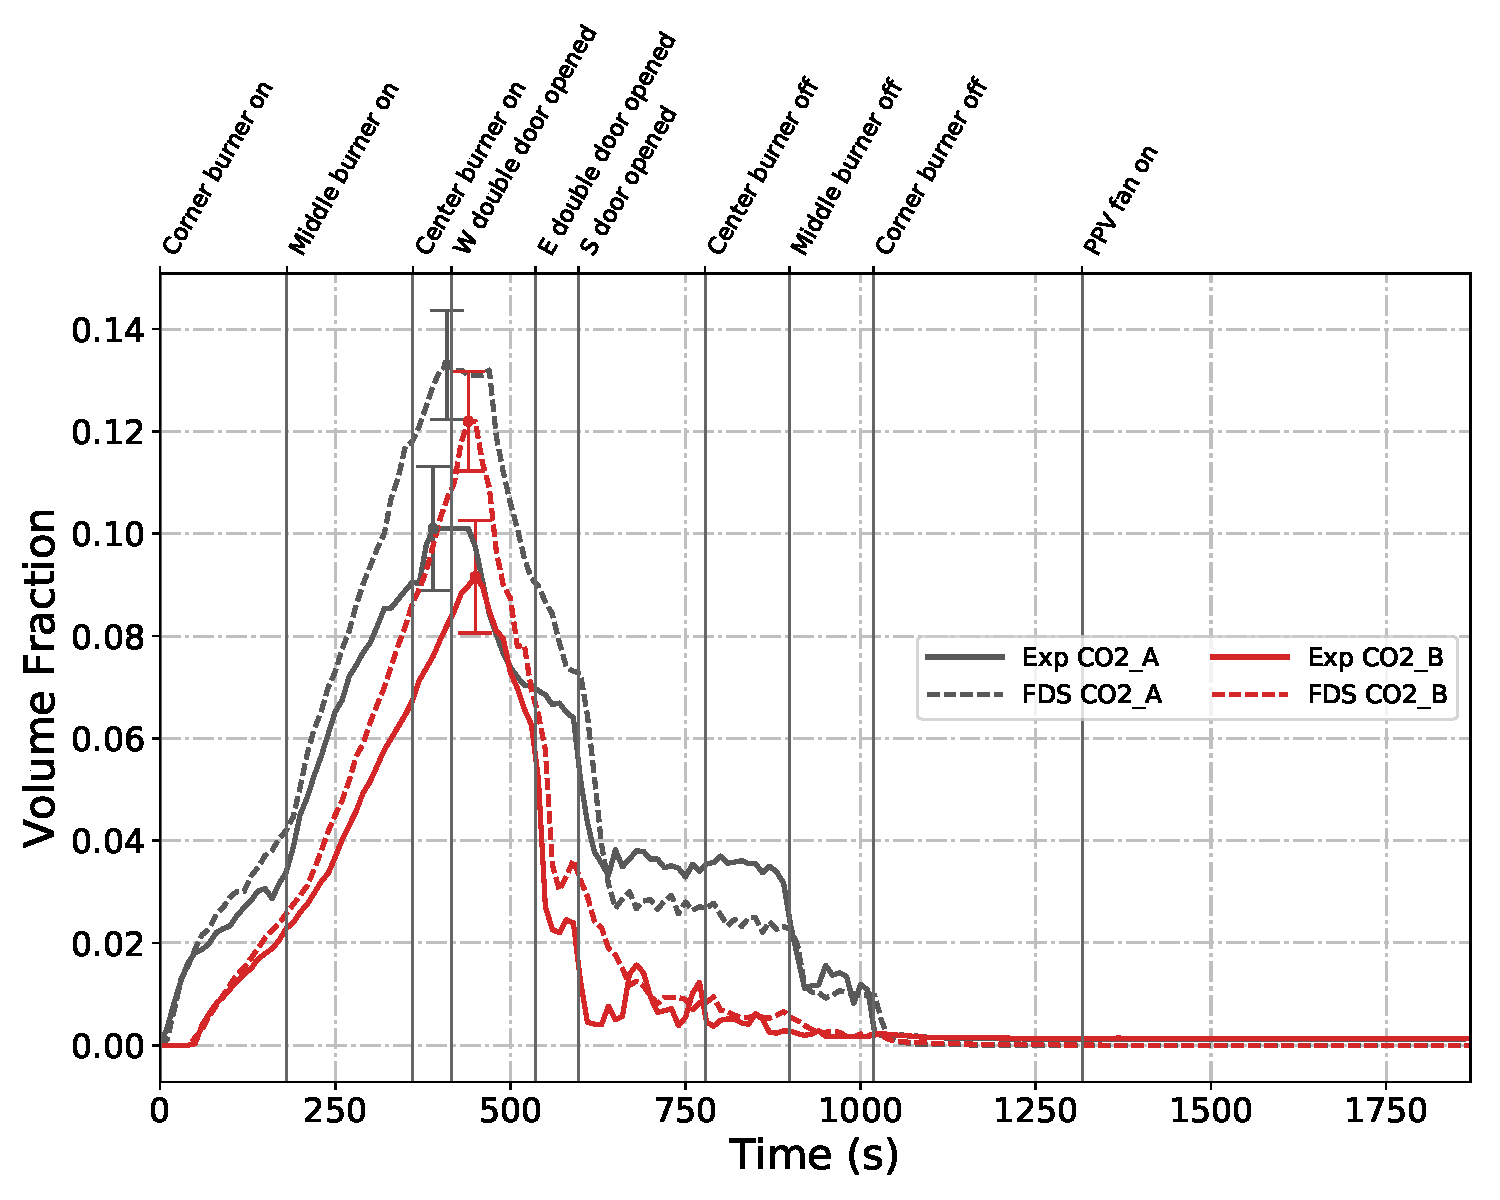
\includegraphics[width=\columnwidth]{Figures/Plots/Validation/Gas_Concentration/Test_3_CO2}
	\caption[Plots of measured and predicted $CO_2$ concentration during Test~3.]{Plots of measured and predicted $CO_2$ concentration in the fire room (black plots) and north room (red plots) during Test~3.}
	\label{fig:Test3_CO2}
\end{figure}

\begin{figure}[!h]
	\centering
	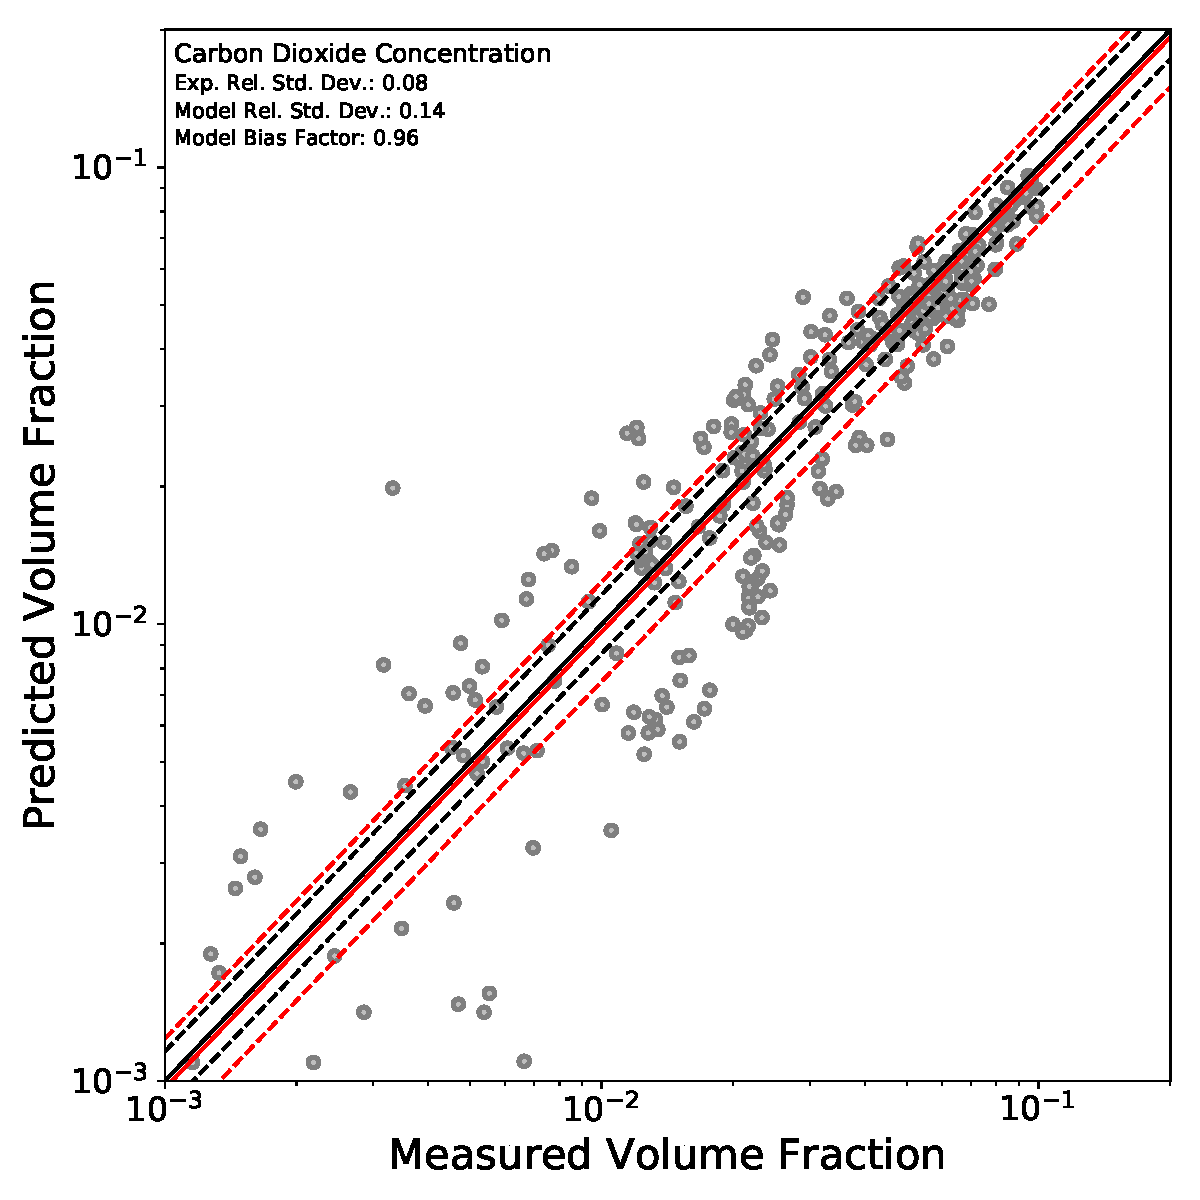
\includegraphics[width=\columnwidth]{Figures/Plots/Validation/Gas_Concentration/loglog_CO2}
	\caption{Summary of measured and predicted $CO_2$ concentrations.}
	\label{fig:loglog_CO2}
\end{figure}

\clearpage
\subsection{Gas Velocity}
Because the gas burner experiments were conducted outdoors, they were subject to environmental conditions, such as wind. To minimize the effect such environmental conditions could have on the analysis of the results, the only gas velocity measurements that are considered in this section are those that were indoors, or well-protected from the exterior. The one gas velocity measurement location in the East Structure that was well-protected from the effects of environmental conditions is the location at the roof vent, the set of three BDPs at the location A10. Tests~5 and 6 were the only East Structure tests that incorporated the roof vent as a ventilation opening. Similarly, there was only one set of BDPs in the West Structure that was well protected from the exterior environment: the set of eight BDPs at the top of the stairs at measurement location A10. All four tests conducted in the West Structure used the stairwell door as a ventilation opening. For Tests~22 and 23, the door was in the open position the entire duration of the experiments, and for Tests~24 and 25, the door was opened at a point during the test. Only the measured and predicted data corresponding to when the door was in the open position is considered in the analysis below. 

\begin{figure}[!h]
	\centering
	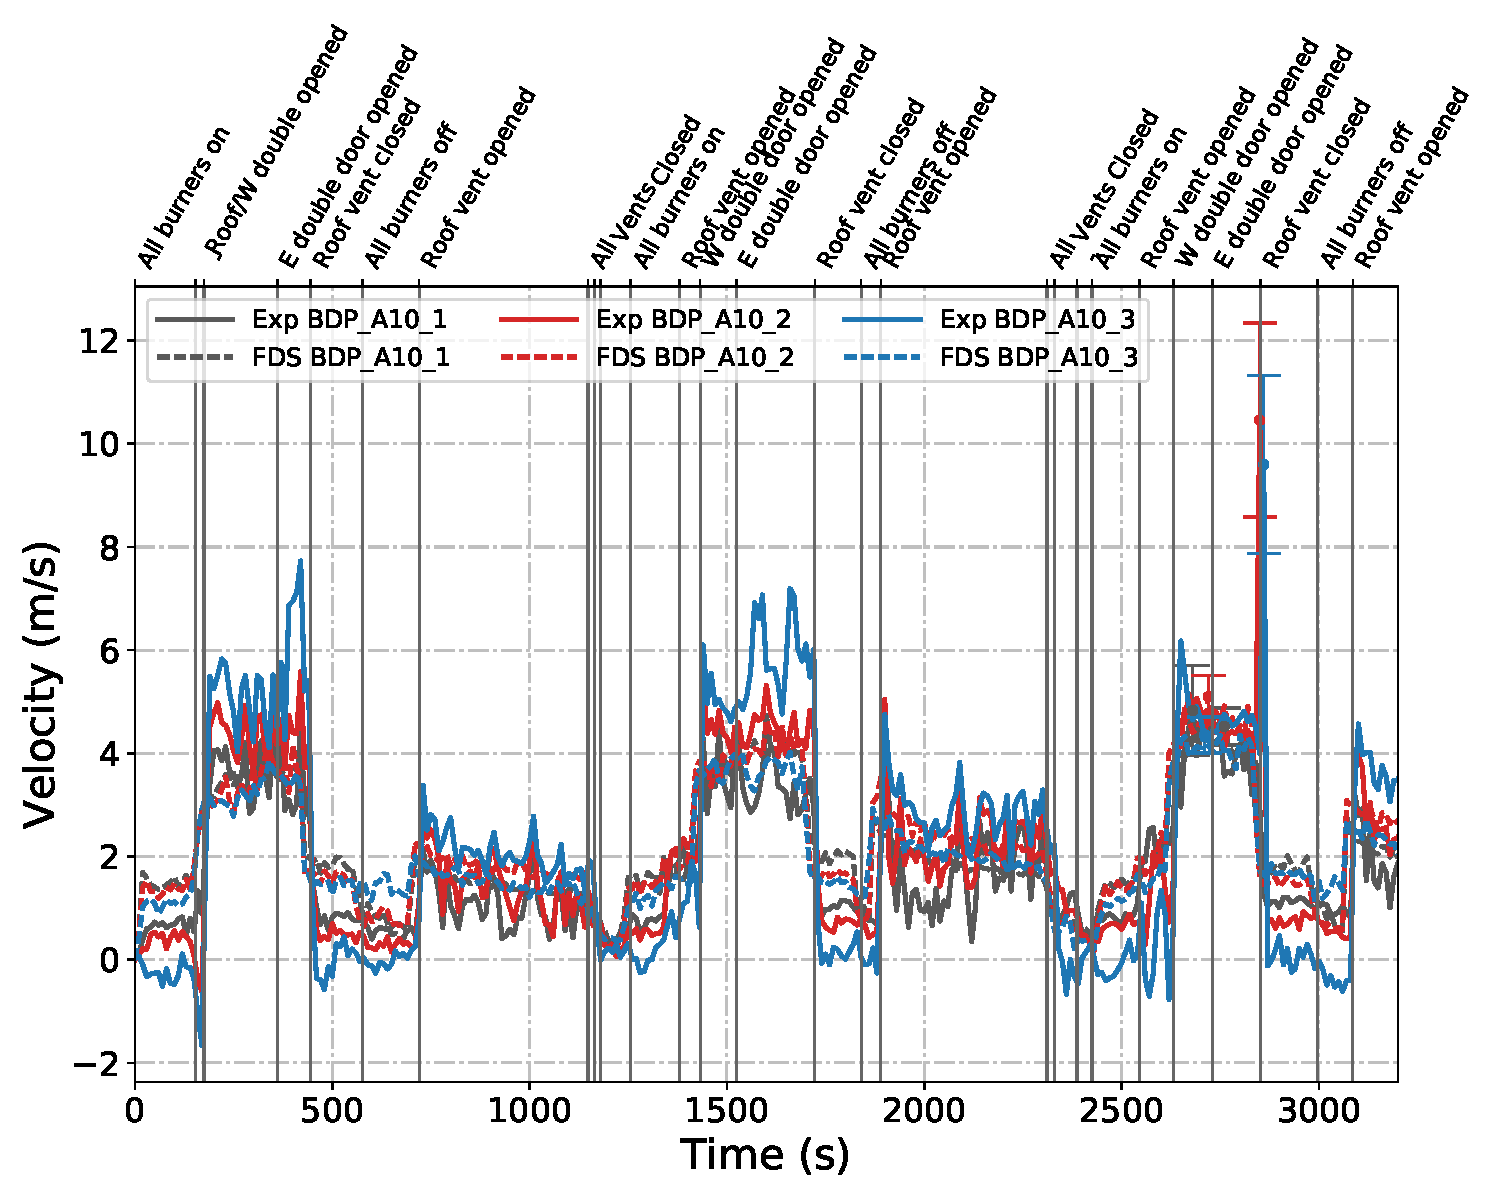
\includegraphics[width=\columnwidth]{Figures/Plots/Validation/Velocity/Test_5_BDP_A10}
	\caption[Plots of measured and predicted gas velocity through the roof vent during Test~5.]{Plots of measured and predicted gas velocity through the roof vent during Test~5.}
	\label{fig:Test5_BDPs}
\end{figure}

\begin{figure}[!h]
	\centering
	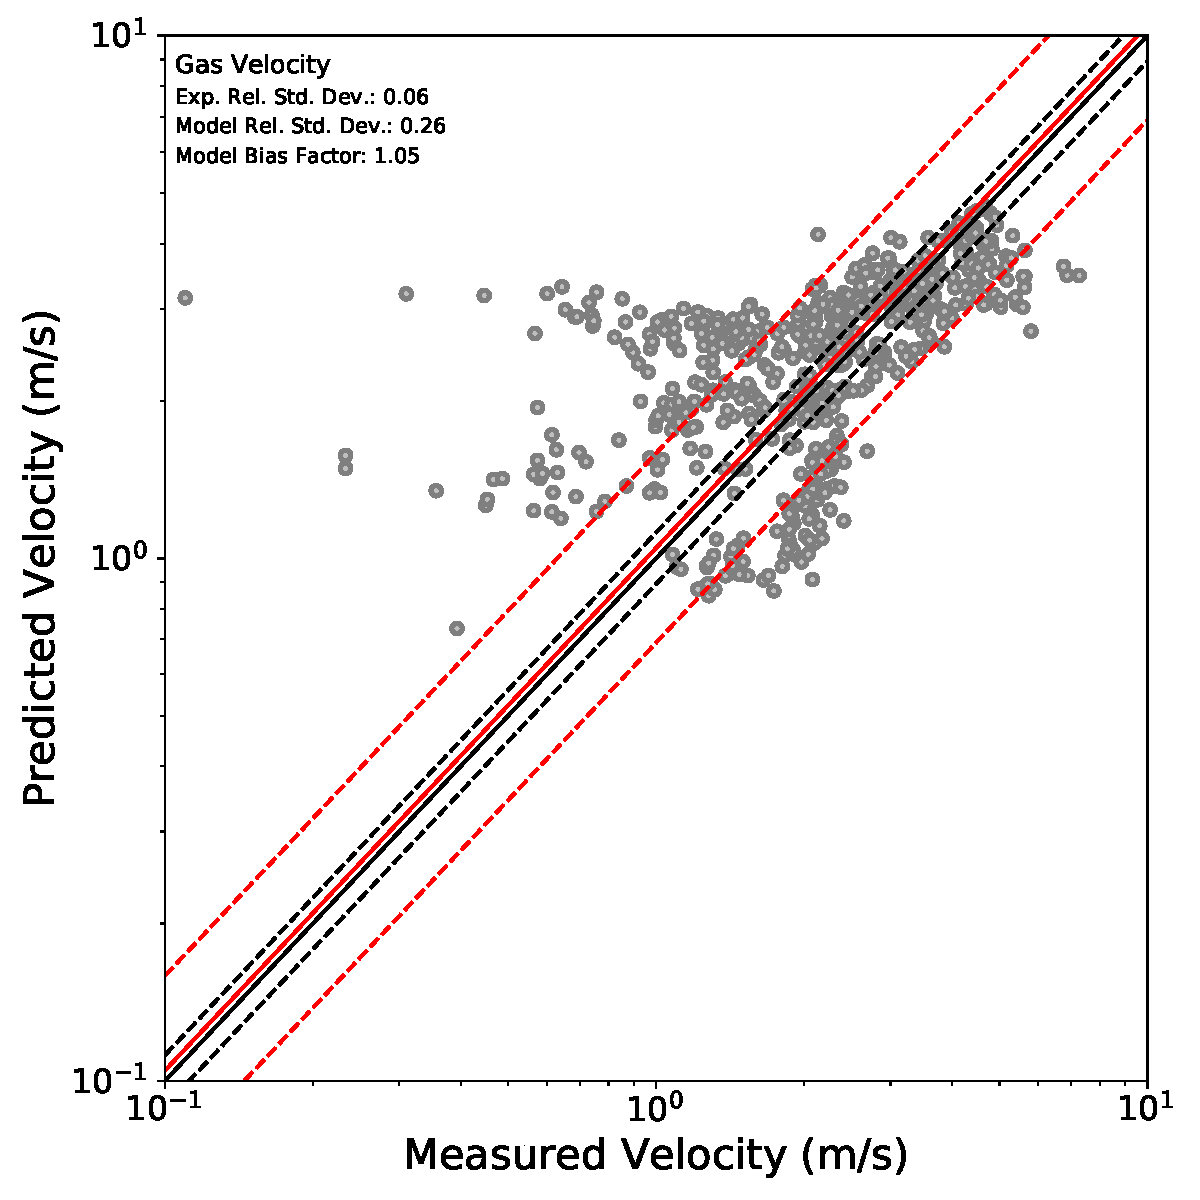
\includegraphics[width=\columnwidth]{Figures/Plots/Validation/Velocity/loglog_BDPs}
	\caption{Summary of measured and predicted gas velocity measurements.}
	\label{fig:loglog_BDPs}
\end{figure}

\clearpage
\subsection{Total Heat Flux}
The heat flux measured by the total heat flux gauges near the stairway door and near the south door on the second floor of the West Structure during Test~23 are plotted with the heat flux data generated by the Test~23 FDS simulation at the same locations in Figure~\ref{fig:Test23_HFs} below. The log/log scatter plot comparing the heat flux data measured by the various heat flux gauges to the heat flux output by FDS at the same locations for the applicable time periods throughout Tests~5--6 and Tests~22--25 is shown in Figure~\ref{fig:loglog_HFs}.  

\begin{figure}[!h]
	\centering
	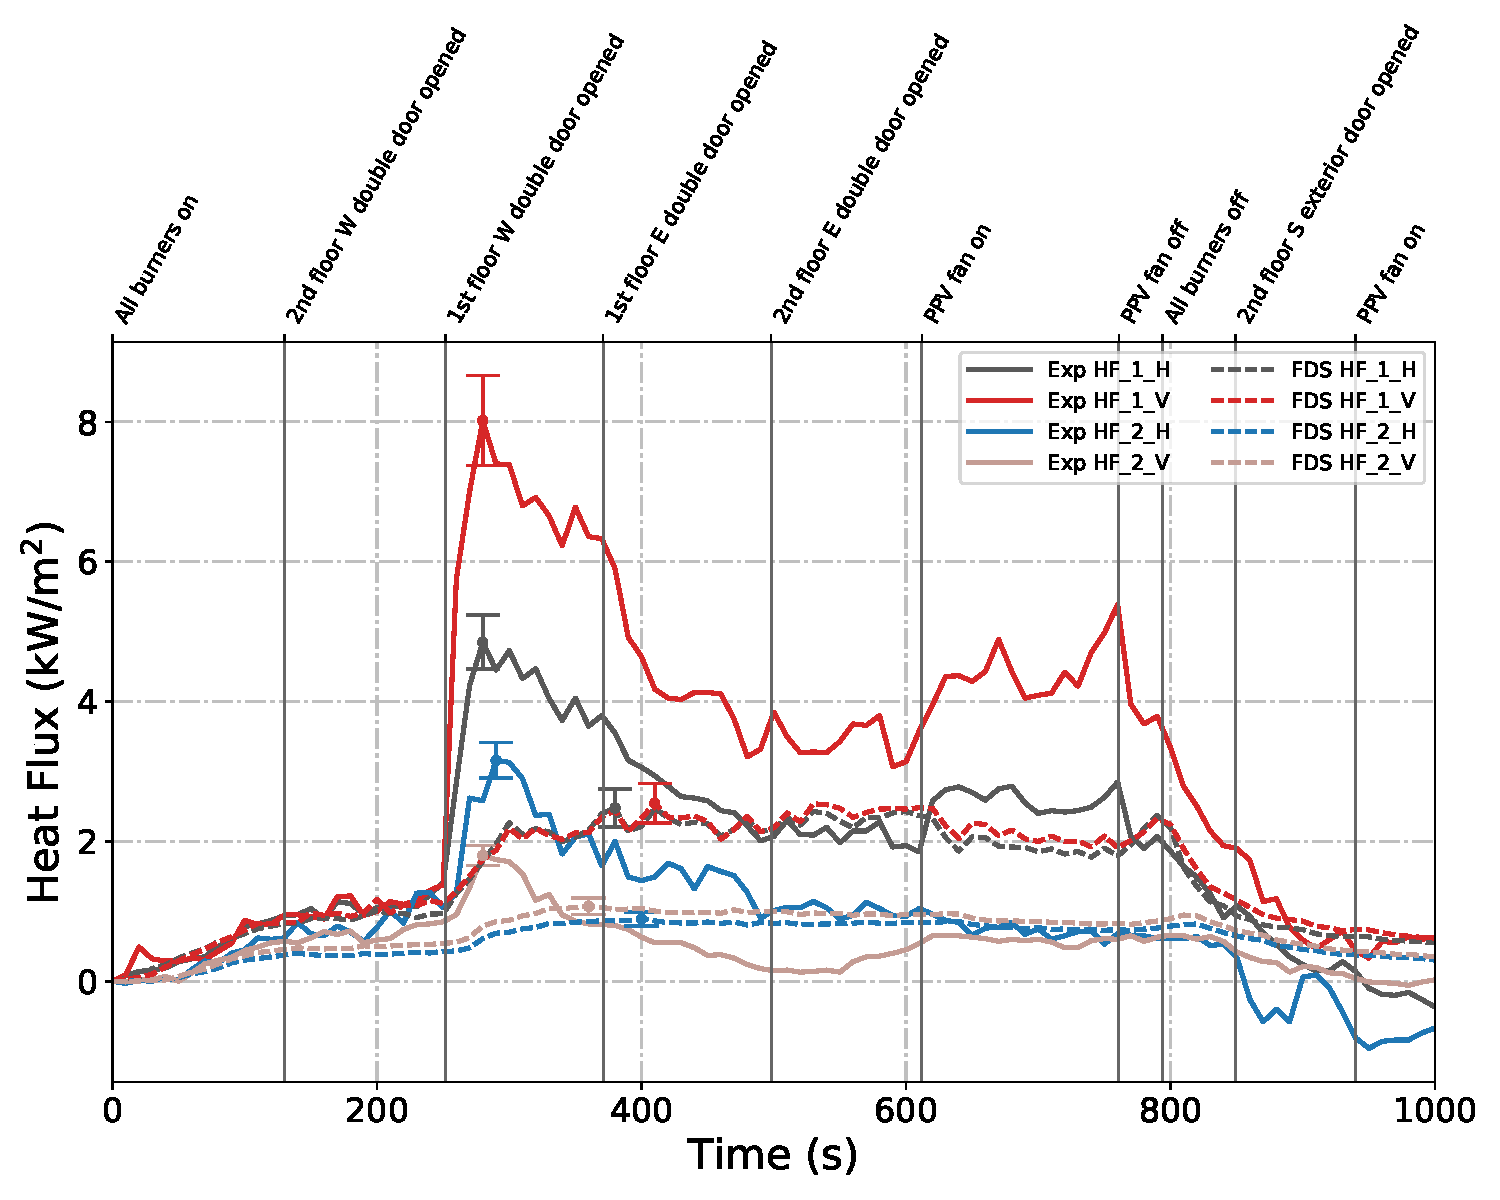
\includegraphics[width=\columnwidth]{Figures/Plots/Validation/Heat_Flux/Test_23_HFs}
	\caption[Plots of measured and predicted heat flux during Test~23.]{Plots of measured and predicted heat flux measured by total heat flux gauges at the top of the stairs facing the stair doorway (`H') and facing the ceiling (`V').}
	\label{fig:Test23_HFs}
\end{figure}

\begin{figure}[!h]
	\centering
	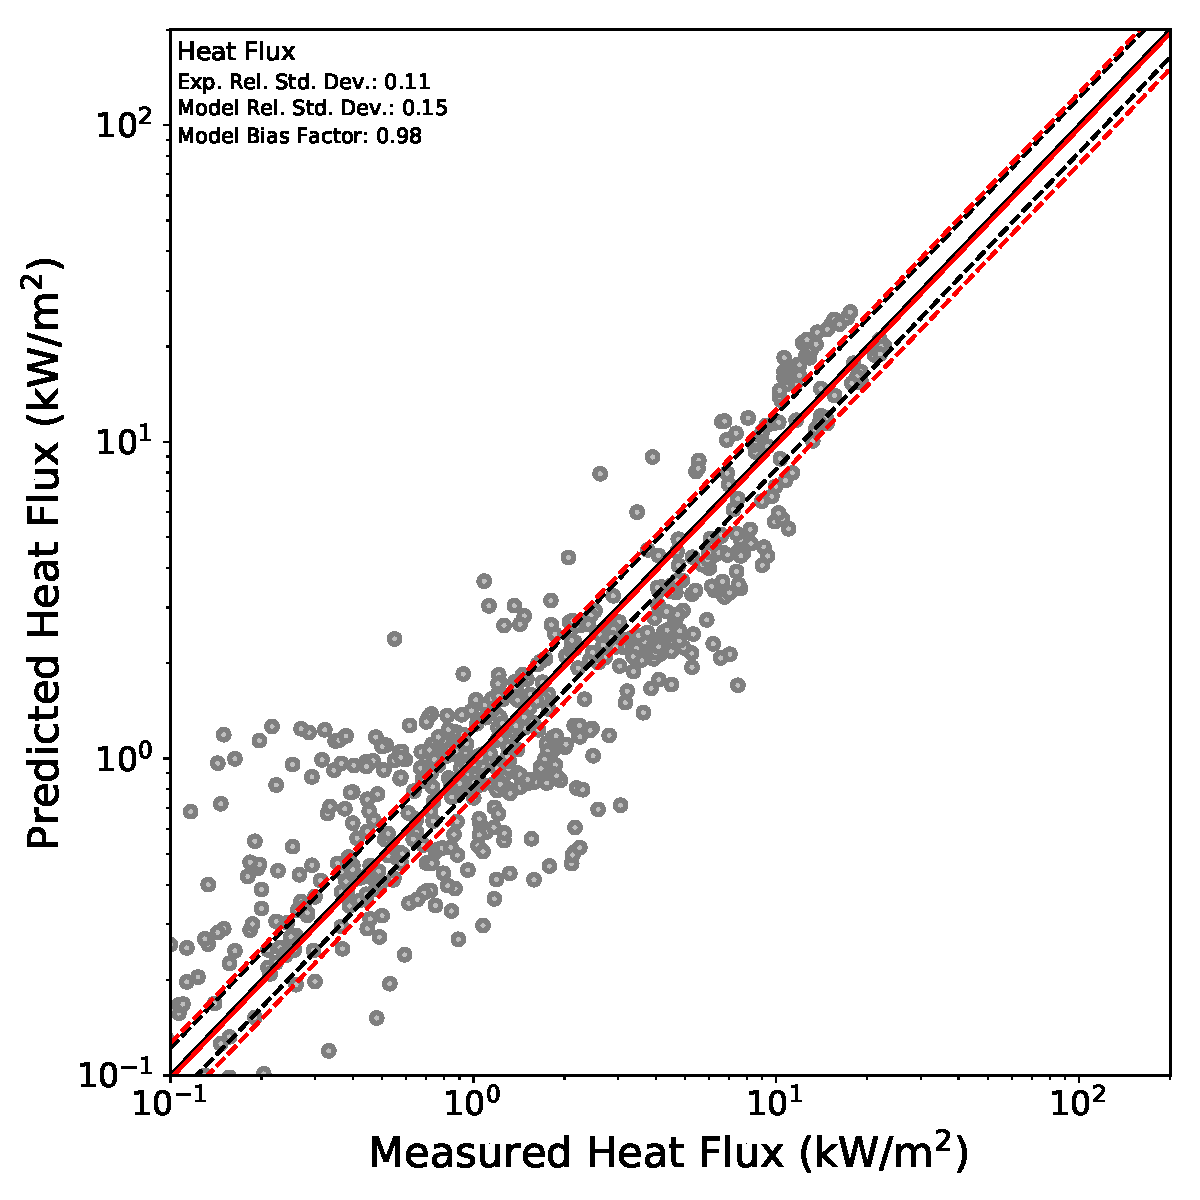
\includegraphics[width=\columnwidth]{Figures/Plots/Validation/Heat_Flux/loglog_HFs}
	\caption{Summary of measured and predicted heat flux measurements.}
	\label{fig:loglog_HFs}
\end{figure}

\clearpage
\subsection{Summary}
Table~\ref{table:stats_compare} compares the model bias factor ($\delta$), the experimental relative standard deviation ($\sigma_E$), and model relative standard deviation ($\sigma_M$) for each data quantity discussed above calculated across all appropriate time durations of the burner experiments to the same values that are listed in FDS Validation Guide for the corresponding data type based on all data within the FDS validation database. 
\begin{table}[!ht]
\caption[Calculated $\delta$, $\sigma_E$, and $\sigma_M$ Values Compared to Values Stated in FDS Validation Guide.]{Comparison of Model Bias Factor ($\delta$) and Relative Standard Deviation of Experimental Data ($\sigma_E$) and Model Data ($\sigma_M$) from all Tests and Same Values Listed in FDS Validation Guide for Each Data Type.}
\begin{center}
\begin{tabular}{lcccccccc}
\toprule
					& & \multicolumn{3}{c}{\textbf{\underline{Calculated}}} & & \multicolumn{3}{c}{\textbf{\underline{FDS Validation}}}   \\
\textbf{Quantity} 	& & \multicolumn{3}{c}{\textbf{\underline{Values}}} 	& & \multicolumn{3}{c}{\textbf{\underline{Guide}}} \\
				 	& & $\delta$ 	&  $\sigma_E$ 	& 	$\sigma_M$ 			& & $\delta$ 	&  $\sigma_E$ 	& 	$\sigma_M$ 		\\	
\midrule
Hot Gas Layer 		& & \multirow{2}{*}{0.97} & \multirow{2}{*}{0.05} & \multirow{2}{*}{0.05} & & \multirow{2}{*}{1.04} & \multirow{2}{*}{0.07} & \multirow{2}{*}{0.07} 	\\
Temperature 		& &					   	  & 					  & 					  & &						& 					   &						\\
\multicolumn{9}{c}{} \\
Ceiling Jet 		& & \multirow{2}{*}{1.03} & \multirow{2}{*}{0.06} & \multirow{2}{*}{0.06} & & \multirow{2}{*}{1.04} & \multirow{2}{*}{0.07} & \multirow{2}{*}{0.13} 	\\
Temperature 		& & 					  & 					  & 					  & &						& 					   &						\\
\multicolumn{9}{c}{} \\
Oxygen 				& & \multirow{2}{*}{1.08}  & \multirow{2}{*}{0.08} & \multirow{2}{*}{0.15} & & \multirow{2}{*}{0.99} & \multirow{2}{*}{0.08} & \multirow{2}{*}{0.14} 	\\
Concentration 		& & 					   & 					  & 					   & & 						& 					   &						\\
\multicolumn{9}{c}{} \\
Carbon Dioxide 		& & \multirow{2}{*}{0.96}  & \multirow{2}{*}{0.08} & \multirow{2}{*}{0.14} & & \multirow{2}{*}{1.00} & \multirow{2}{*}{0.08} & \multirow{2}{*}{0.12} 	\\
Concentration 		& & 					   & 					  & 					   & & 						& 					   &						\\
\multicolumn{9}{c}{} \\
Gas Velocity 		& & 1.05  & 0.06 & 0.26 & & 0.99 & 0.08 & 0.09 	\\
\multicolumn{9}{c}{} \\
Heat Flux 			& & 0.98  & 0.11 & 0.15 & & 0.98 & 0.11 & 0.24 	\\
\bottomrule
\end{tabular}
\end{center}
\label{table:stats_compare}
\end{table}

Overall, the agreement between the FDS simulation data and experimental data for the gas burner experiments is consistent with the statistical values given by the FDS Validation Guide. For the hot gas layer temperature, ceiling jet temperature, and heat flux, the model bias calculated for the gas burner simulations is equal to or better than (closer to the ideal value of 1) the overall model bias values given by the FDS Validation Guide. Additionally, the relative standard deviations of the experimental data and model data for these three quantities are equal to or less than (better than) the corresponding values for the same data types listed in the validation guide. 

The $\delta$, $\sigma_E$, and $\sigma_M$ values produced by the gas burner model and experimental data for both the $O_2$ and $CO_2$ gas concentrations were very close to the values documented in the FDS Validation Guide. The $\sigma_E$ values are equal in both comparisons and the $\sigma_M$ values are greater in magnitude by only 0.01 and 0.02 compared to the validation guide values for oxygen and carbon dioxide concentration, respectively. Finally, based on the data from gas burner simulations, the oxygen concentration model bias is worse (further from the ideal value of 1) by 7~\% and carbon dioxide concentration model bias is worse by 4~\% compared to the documented values in the FDS Validation Guide.

The most significant discrepancy between the documented values and values from the gas burner models is seen in the gas velocity comparison, in which $\sigma_M$ was calculated as being greater than the $\sigma_M$ from the validation guide by a value 0.18. This discrepancy may exist for a few of reasons. First, gas velocity was one of the quantities with the highest uncertainty associated with the experimental measurements. Also, as previously mentioned, the experiments were conducted outdoors, so environmental conditions may have affected the measurements, even though only data from BDPs that were fully inside the structures were considered. All the tests used to calculate the $\delta$, $\sigma_E$, and $\sigma_M$ within the validation guide were conducted in an indoors laboratory setting, which could explain the significantly smaller model relative standard deviation. Finally, due to the nature of the fire environment at the time of the measurements, it's possible that turbulent flow was occurring through the vents (especially the roof vent in Tests~5 and 6) at the time of the measurements. LES CFD models, like FDS, tend to be limited more in terms of accurately measuring turbulent flow than compared to measurements during other conditions.
